%Chapter 6

\renewcommand{\thechapter}{6}

\chapter{Enhancing optical nonlinearity through \texorpdfstring{\\}{ }microcavity system }
\label{chap6}

\section{Introduction}
% An emerging field of quantum nonlinear optics seeks to achieve strong nonlinearity with lower power and ultimately even at the few-photon level. 
% This has been a significant goal in both classical and nonclassical optics, as it enables energy-efficient devices such as optical switches, single-photon transistors, and gates~\cite{ref1,ref2,ref3,ref4}. 
% However, photons, as the fundamental units of light, generally do not interact with each other unless under very specific conditions. 
% One approach to facilitate strong photon--photon interactions is by integrating materials with strong nonlinearities. 
% For example, systems such as single atoms~\cite{ref5,ref6}, molecules~\cite{ref7}, and atomic defects in solids~\cite{ref8}, where the reflectance and absorption of the particle can be modified by a single photon with inherently strong nonlinearities. 
% Such nonlinearity can be considered as, for instance, third-order nonlinearities such as saturable absorption with a saturation intensity corresponding to one photon per lifetime~\cite{ref9}. 
% However, a major challenge to demonstrate single-photon nonlinearity lies in the deterministic coupling of light to these emitters, such as embedding them in optical resonators~\cite{ref4,ref5,ref6,ref10}. 

% An alternative approach involves using extended optical excitations, such as excitons in semiconductors. 
% Excitons have larger oscillator strengths, which lead to stronger coupling to light, making them a promising candidate for achieving the desired nonlinear interactions~\cite{ref11}. 
% The exciton density-dependent resonance leads to third-order nonlinearity, which can be both dispersive and dissipative. 
% The challenge, however, lies in the relatively weak nonlinearities due to the weak interactions among excitons that are charge neutral. 
% For instance, in 2D semiconductors such as monolayer MoSe$_2$~\cite{ref12}, the excitonic nonlinearity induced by the exciton--exciton interaction can be observed as exciton blueshift under pulsed laser excitation. 
% The interaction strength, $g_{\mathrm{exc}}$, is defined as the energy shift induced per unit area density of excitons. 
% Rather generally, the exciton--exciton interaction $g_{\mathrm{exc}}$, dominated by exchange interactions, is on the order of $\sim E_B R_b^2$, where $E_B$ is the exciton binding energy and $R_b$ is the exciton Bohr radius. 
% Notably, a smaller Bohr radius leads to tighter binding of excitons, which makes $g_{\mathrm{exc}}$ more or less agnostic of materials, on the order of $\sim \mu$eV$\cdot\mu$m$^2$, whether in TMDs or GaAs quantum wells~\cite{ref13}.

% Given the intrinsically weak exciton--exciton interactions, various strategies are being pursued to enhance nonlinearity to the few-photon regime. 
% A prominent approach involves integrating optical materials with cavities or waveguides~\cite{ref19,ref20}. 
% For example, embedding TMDs into optical cavities leads to the formation of exciton--polaritons---a state that is half-light and half-matter---when the energy exchange between photons and excitons occurs faster than their respective decay rates. 
% This strong light--matter coupling is typically characterized by the emergence of two polariton states with distinct energies---lower and upper polaritons~\cite{ref21}. 
% The coupling strength, also known as vacuum Rabi splitting, can be determined by observing the anti-crossing behavior between excitons and photons. 
% Crucially, polaritons often exhibit different nonlinear responses compared to bare excitons. 
% In particular, the nonlinearity of polariton can be expressed as the susceptibility:  
% \begin{equation}
% \chi^{(3)}(r) = \frac{16 g_{\mathrm{exc-ph}}^{4}}{|\Gamma|^{2} \Gamma} \cdot \frac{i U(r)}{\Gamma + i U(r)} 
% \label{eq:susceptibility}
% \end{equation}
% where $g_{\mathrm{exc-ph}}$ is the coupling strength between exciton and photon, $U(r)$ is the interaction strength between two excitons at distance $r$, and $\Gamma$ is the linewidth. 
% Meanwhile, the cavity modifies the linewidth of the excitons, often reducing the number of photons required to shift the resonance by a linewidth.  

% Last but not least, with increasing pumping intensity, the vacuum Rabi splitting between the two polaritons also decreases, leading to the energy shift of polaritons~\cite{ref22,ref23}. 
% The reduction in the splitting is due to phase-space filling~\cite{ref24}, where more exciton population leads to fewer excitons left to couple to the cavity photon, similar to saturable absorption. 
% In fact, the Rabi splitting strength $\Omega$ depends on the polariton density:  
% \begin{equation}
% \Omega = 2g \left(1 - \frac{n \pi R_b^2}{2}\right)
% \label{eq:rabi}
% \end{equation}
% which leads to a phase-space-filling-induced nonlinearity, with the strength quantified as $g_{\mathrm{pol-pol}} \propto a_b^2 \hbar \Omega$~\cite{ref25}.
% At low density, the exchange interactions from the excitonic component dominate the polariton nonlinearity, resulting in a blue shift of both polariton branch resonances~\cite{ref26}.  

% TMDs offer several appealing features for exploring the nonlinear interaction of polaritons in the strong light--matter coupling regime. 
% With excitons in TMDs possessing large binding energies ranging from 200 to 500~meV and large oscillator strengths, strong coupling can persist even at room temperature with possibly enhanced exciton-mediated nonlinearity~\cite{ref27}. 
% The nonlinearity of polaritons generated in TMDs varies significantly depending on the specific species coupled to the cavity photon. 
% In monolayer WSe$_2$, the 2s exciton--polaritons exhibit a larger nonlinearity of approximately $46.4 \pm 13.9~\mu$eV$\cdot\mu$m$^2$, which is about four times larger than that of the 1s state~\cite{ref24}. 
% This difference is expected, given the larger Bohr radius of the 2s exciton. 
% Biexciton polaritons also exhibit a nonlinear interaction boost~\cite{ref28}. 
% Phase-space filling was thought to play an important role in the measured nonlinear response in TMD polaritons. 
% Similarly, trion--polaritons in monolayer MoSe$_2$ microcavities exhibit enhancement of the nonlinearity strength of $\sim 37 \pm 3~\mu$eV$\cdot\mu$m$^2$ at a low electron density and pump fluence~\cite{ref29}, driven by the strong band-filling effect. 
% However, the increased nonlinearity observed in 2s exciton- and trion-polaritons comes at the cost of reduced coupling strength between the optical excitation and the photons due to their weaker oscillator strength.  

% Another approach uses interlayer excitons with stronger dipolar repulsion, such as those in bilayer MoS$_2$~\cite{ref15}. 
% Such interlayer excitons can have sufficient oscillator strength to enable strong coupling when the carrier tunneling in the material is large enough to produce hybridization between interlayer and intralayer states~\cite{ref30}. 
% Combining this IX exciton with cavity photons forms the dipolar interlayer polariton, which has a ten-fold enhancement of the nonlinearity strength ($g_{\mathrm{IX}} \sim 100 \pm 2~\mu$eV$\cdot\mu$m$^2$) compared with the conventional intralayer exciton ($g_A \sim 10 \pm 0.2~\mu$eV$\cdot\mu$m$^2$) embedded in a microcavity~\cite{ref15,ref31}.  

% An intriguing set of recent experiments uses the moiré superlattice in 2D materials to demonstrate strong nonlinearity in exciton--polariton systems~\cite{ref32}. 
% With the moiré excitons confined within each site, they experience strong on-site interactions~\cite{ref33,ref34,ref35}, which suggests that exciton blockade can occur when the average exciton--exciton density is close to the size of the moiré cell, on the order of a few to tens of nanometers, much larger than the blockade radius of bare excitons. 
% Meanwhile, the exciton and photon can still couple collectively among all the cells, which maintains the system in a strong coupling regime.  

% With the above developments, it has become more feasible for this system to finally enter the quantum nonlinear optics regime when the polariton nonlinear interaction strength surpasses the linewidth. 
% In such a case, the optical response of the system is significantly altered by the presence of a single photon, leading to unprecedented phenomena and technologies in solids. 
% One example is the so-called photon blockade~\cite{ref36,ref37}, where a single polariton can inhibit the transmission of additional photons. 
% Such photon blockade effects can be observed through photon antibunching and could open exciting avenues for realizing nonclassical light sources in quantum nonlinear optics~\cite{ref38,ref39,ref40,ref41}.  

Strong optical nonlinearities at the few-photon level are highly sought after for energy-efficient photonic and quantum devices, such as all-optical switches, transistors, and gates~\cite{Hwang2009-rg,Turchette1995-nv,Chang2007-lw,Volz2012-pb}. 
Yet photons do not naturally interact, and achieving such effects requires materials or systems with enhanced nonlinear responses.  

Early approaches used individual quantum emitters such as atoms, molecules, or defects, where a single photon can substantially alter absorption or reflectance~\cite{Birnbaum2005-ix,Schuster2008-nv,Lounis2000-iy,Castelletto2014-pv}. 
While these systems demonstrate strong nonlinearities, their practical use is limited by the challenge of deterministically coupling photons to isolated emitters~\cite{Harris1990-ej,Fushman2008-lk}.  

Excitons in semiconductors offer a collective platform, with large oscillator strengths that enable strong light--matter coupling\cite{Wang2018-my}.
However, because excitons are charge neutral, their mutual interactions are relatively weak, producing nonlinearities on the order of only a few $\mu$eV$\cdot\mu$m$^2$ across both TMDs and quantum wells~\cite{Scuri2018-bn,Shahnazaryan2017-gx}.  

Embedding excitons in optical cavities forms exciton--polaritons, hybrid light--matter quasiparticles that inherit both strong coupling and nonlinear response~\cite{Liu2015-hm,Deng2010-ul}. 
Compared with bare excitons, polaritons show enhanced nonlinearities due to modified linewidths and collective light--matter interactions. 
The polariton nonlinear shift can be contributed from the exciton-exciton interaction at lower exciton population desntiy\cite{Gu2021-cu,Ciuti2003-zj} and phase-space filling,
where exciton saturation reduces the available oscillator strength~\cite{Song2024-na,Gu2021-cu}.  

TMD monolayers provide an especially attractive platform due to their large binding energies (200--500 meV) and strong oscillator strengths, enabling robust polariton formation even at room temperature~\cite{Wang2018-my}. 
Recent studies have reported enhanced nonlinearities in higher-order exciton states, biexcitons, and trions~\cite{Gu2021-cu,Wei2023-by,Emmanuele2020-oh}, though these gains can come at the cost of weaker light coupling. 
Interlayer excitons, with their strong dipole--dipole repulsion, and moiré-confined excitons further offer routes to boost polariton interactions by an order of magnitude or more~\cite{Datta2022-po,Leisgang2020-mn,Louca2023-in,Zhang2021-eb}.  

These advances suggest that exciton--polaritons in 2D materials are a promising pathway toward the quantum nonlinear optics regime, where the interaction strength exceeds the linewidth. 
In this limit, a single polariton can block the transmission of others, giving rise to photon blockade and enabling nonclassical light sources~\cite{A-Verger-C-Ciuti-and-I-Carusotto2006-wd,Munoz-Matutano2019-cg,Somaschi2016-uk,He2013-od,Turunen2022-wom,Delteil2019-pp}.  

In this work, we present a method to utilize a 1D microcavity with highly confined photons to couple with the Fermi polaron in homotrilayer WSe$_2$, aiming to further enhance the nonlinearity and reduce the number of photons required for photon blockade. 
We first designed this high-quality microcavity with highly reflective dielectric Bragg mirrors (TiO$_2$ and SiO$_2$) for the designed wavelength of light (730~nm). 
We then embed the trilayer WSe$_2$ device with monolayer/bilayer graphene as dual gates into this microcavity. 
Thanks to the large oscillator strength of the excitons and polarons in the trilayer WSe$_2$, we can enter a strong coupling regime between the exciton/polaron and the photon---indicated by the signature of the formation of polaritons, which can be tuned by electrical gating.

\section{Design of gate compatible 1D microcavity}
\subsection{Cavity simulation}
Embedding TMDs or other 2D materials with a 1D microcavity has already been demonstrated~\cite{cite}. 
However, the overall quality factor of the cavity can be low due to the large inhomogeneous nature of the van der Waals structure. 
As a result, gate-dependent control of polaritons is seldom studied, as the gating material graphite has high optical loss, and adding it to the structure would further reduce the $Q$ value. 

Here, we tune the position of the graphite gate. 
By placing the graphite at the mode field minimum, the cavity loss can be greatly reduced. 
As shown in the schematic below, the total cavity length $l$ is given by the total thickness of the van der Waals stack. 
The cavity length is expressed as $l = \frac{m \lambda_{0}}{2 n_{\mathrm{hBN}}}$,
where $m$ is the mode number inside the cavity. 
For a mode value of $m=5$, we need four layers of hBN: two of them with thicknesses $l_{\mathrm{gr1}}$ and $l_{\mathrm{gr2}}$, and the other two with thicknesses of $\frac{1}{2} l_c$. 
Placing graphite at the node of the field gives the distance 
$l_{\mathrm{gr1}},\, l_{\mathrm{gr2}} = \frac{n \, l}{m}$ and the condition  
$l_{\mathrm{gr1}} + l_{\mathrm{gr2}} + l_c = l$.

%Fig.6.1--------------
% \vspace{1em}
\renewcommand{\baselinestretch}{1}
\small\normalsize
\begin{quote}
\begin{figure}[htbp]
\begin{center}
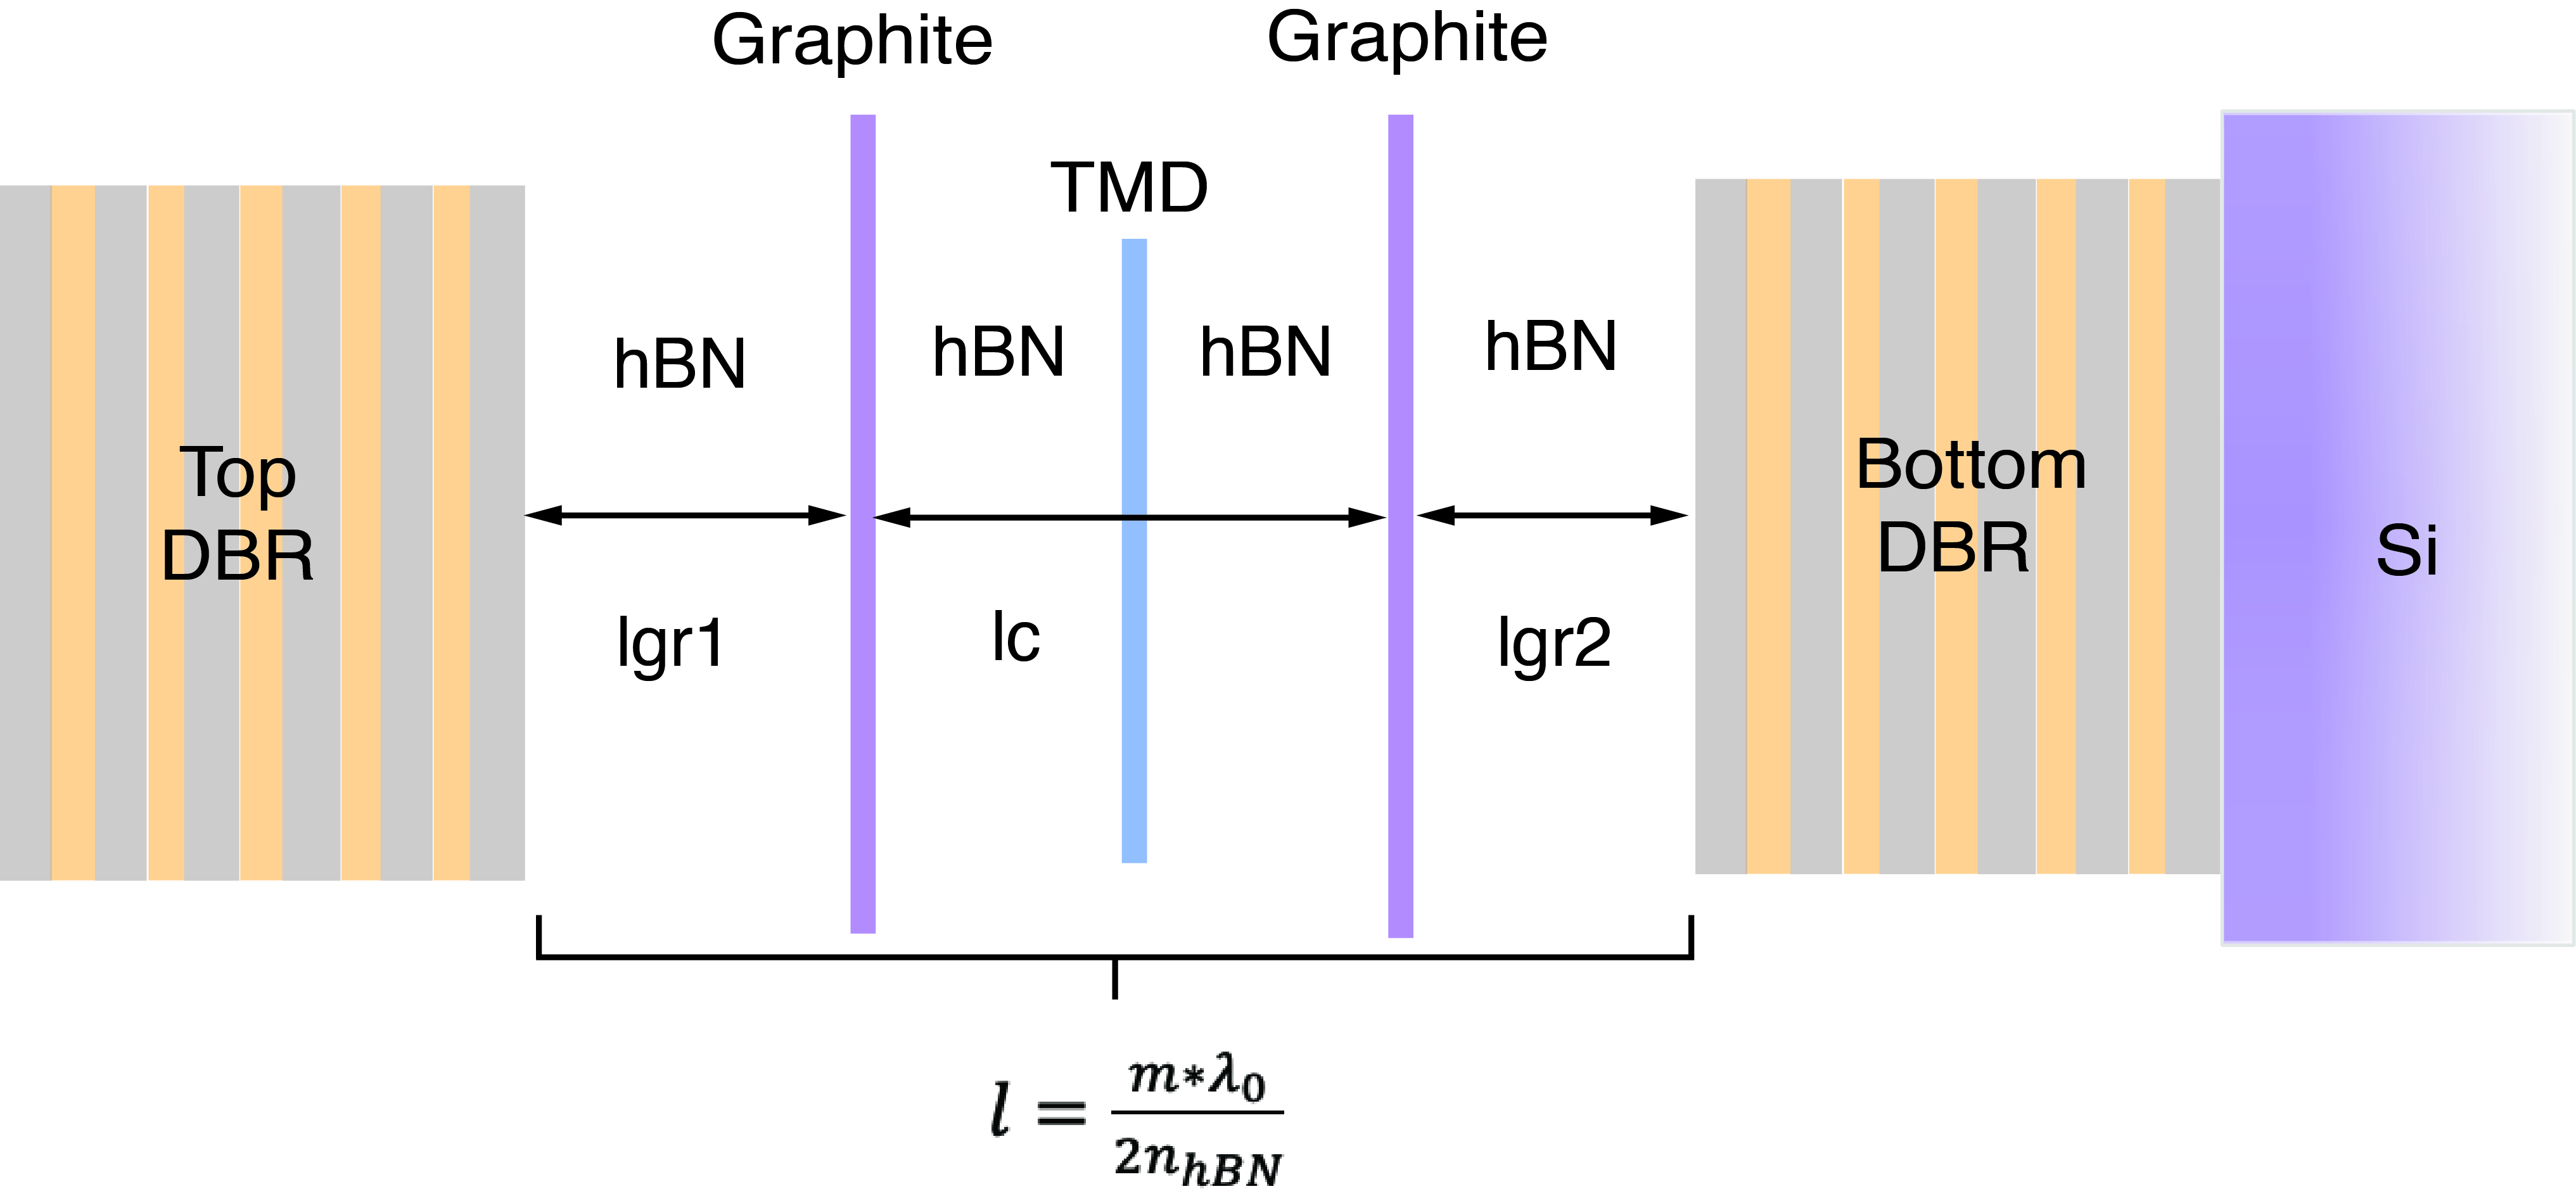
\includegraphics[width=0.7\textwidth]{Figures/C6/Fig6.1.jpg} % 
\end{center}
\caption[Schematic of van der Waals 1D microcavity design.] 
{\textbf{Schematic of van der Waals 1D microcavity design.}}
\label{fig.6.1}
\end{figure}
\end{quote}
\renewcommand{\baselinestretch}{2}
\small\normalsize
% %/////////////////////// 
Then by using the Transfer Matrix Method (TMM) with the optical indices of all constituent materials (hBN, graphite) and the thickness of each layer, we can simulate the field distribution and optimize the $Q$-factor of our proposed microcavity structure. 
Figure~\ref{fig.6.1} shows the schematic and the simulated reflectance spectrum of the microcavity with the embedded van der Waals stack (without TMD). 
According to our simulation, the cavity achieves a $Q$-factor of approximately 2500 at normal incidence (Figure~\ref{fig.6.2}).

%Fig.6.2--------------
% \vspace{1em}
\renewcommand{\baselinestretch}{1}
\small\normalsize
\begin{quote}
\begin{figure}[htbp]
\begin{center}
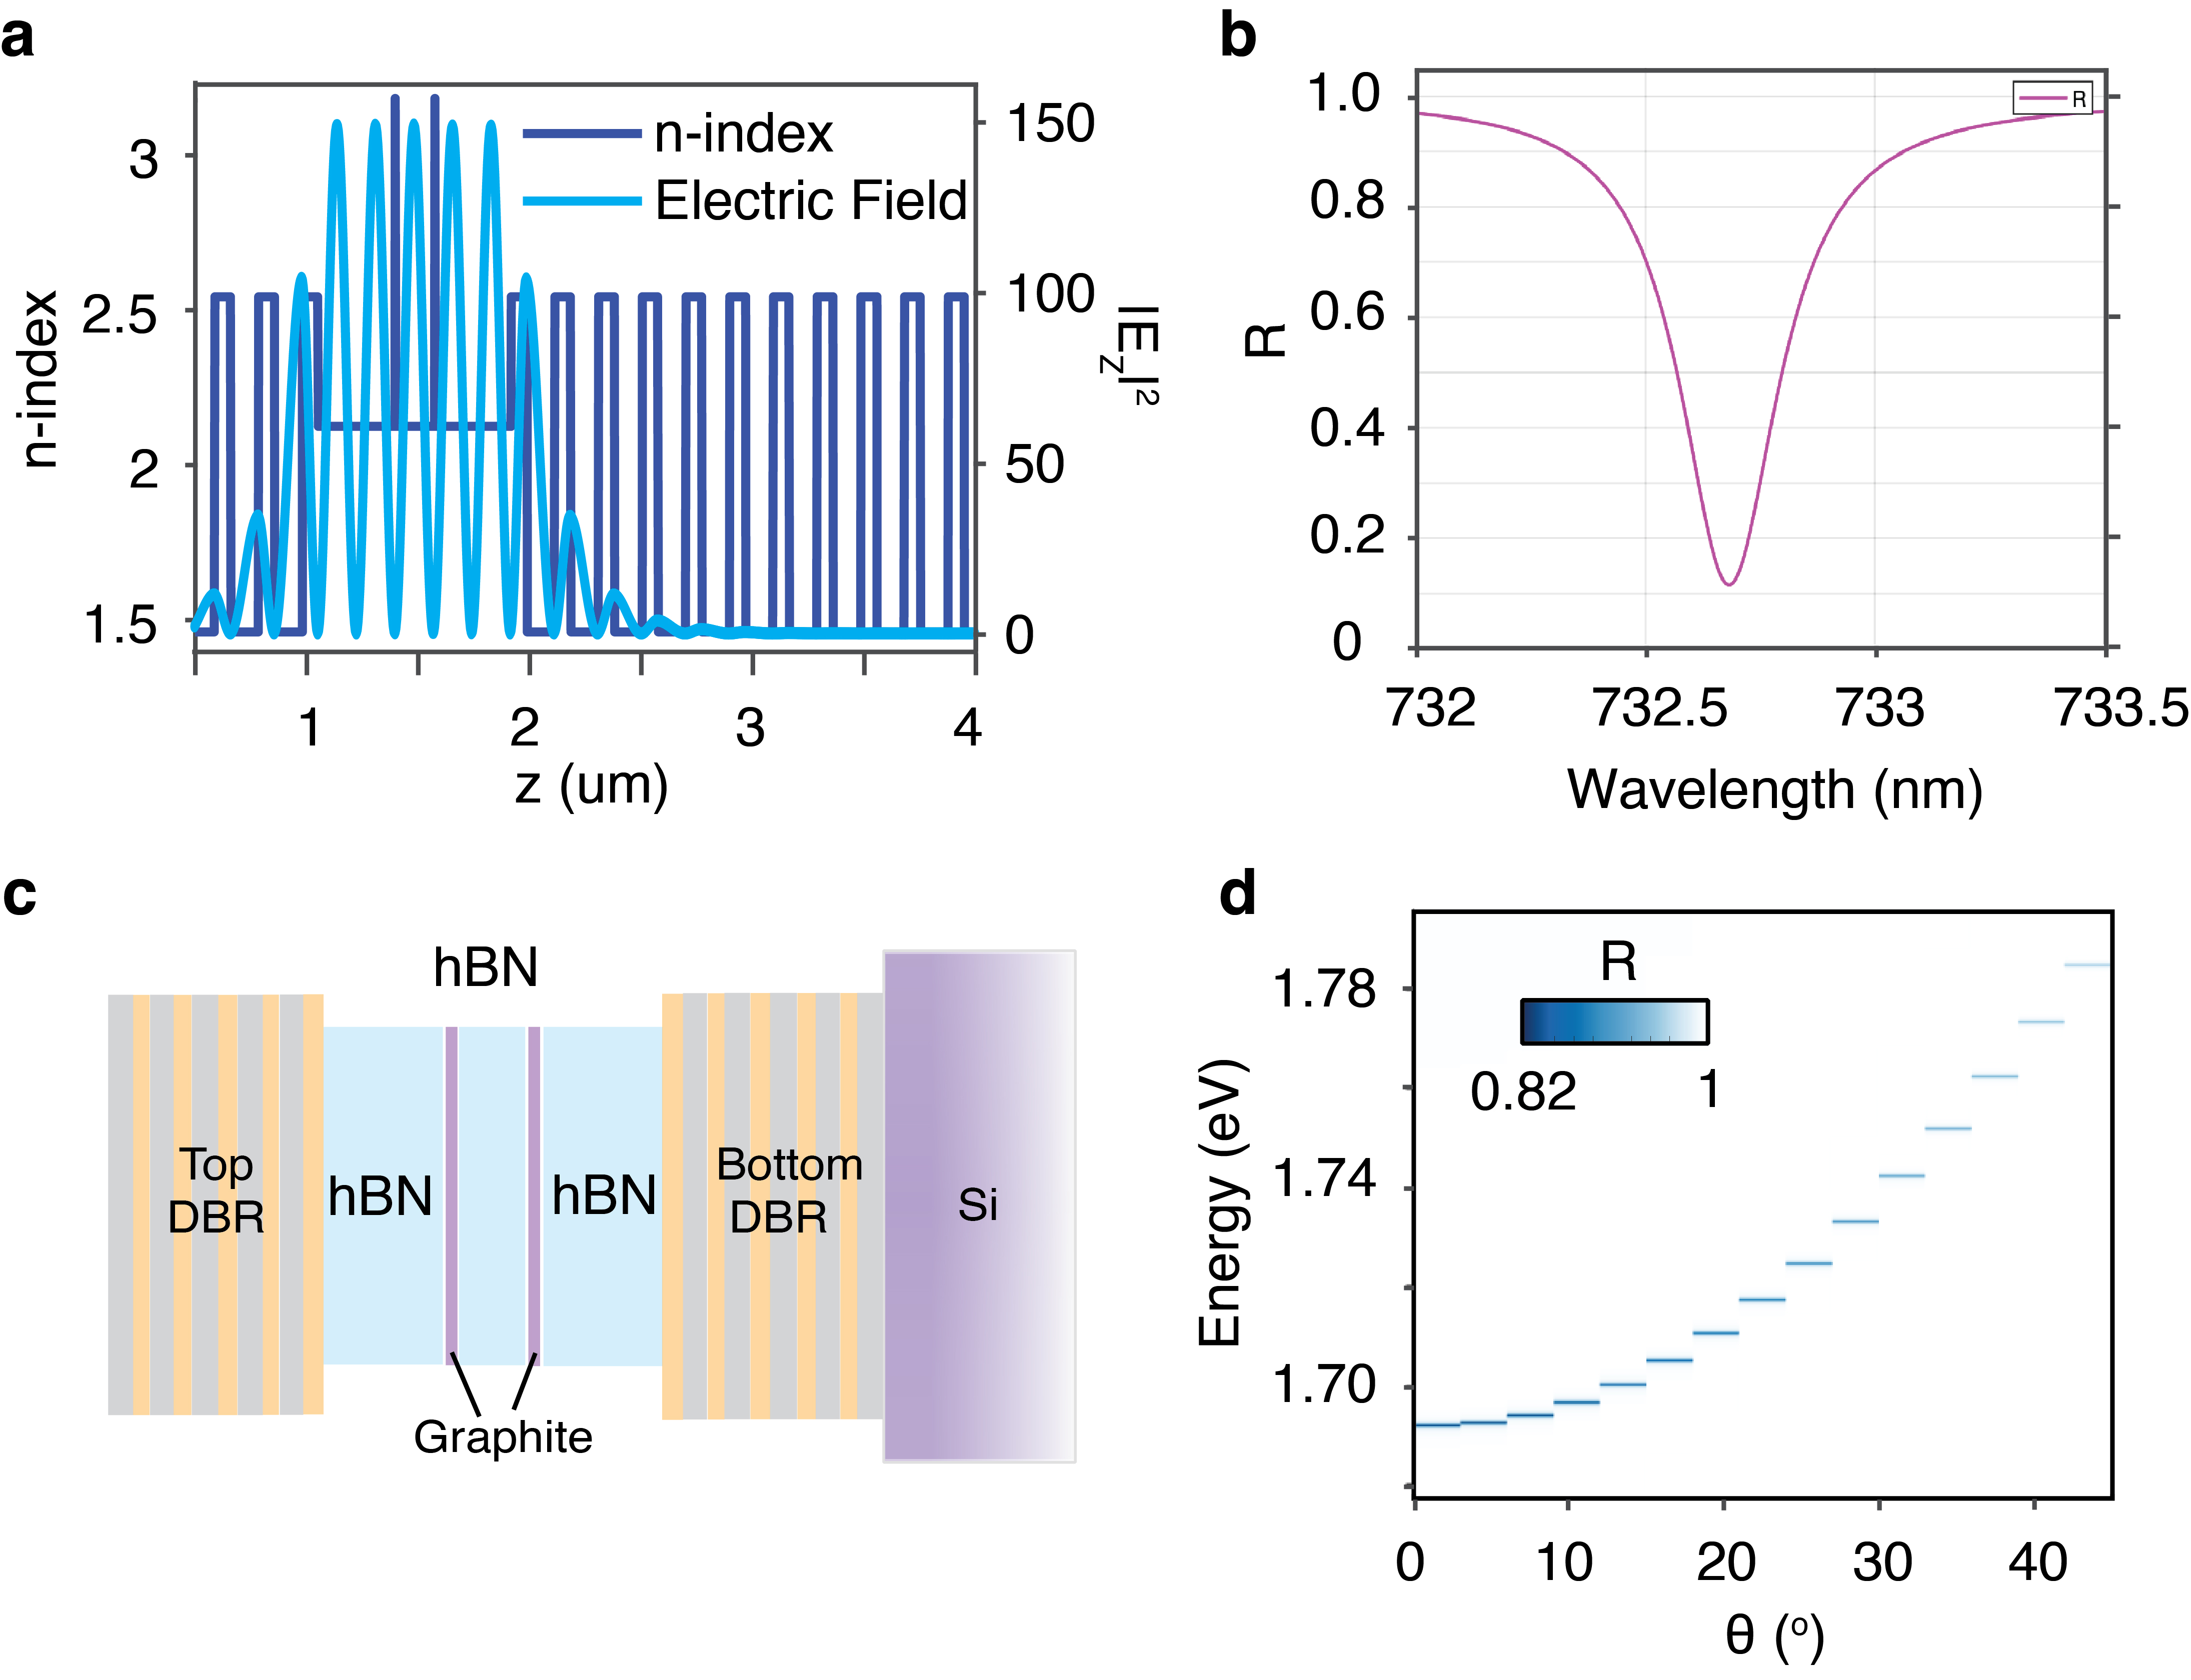
\includegraphics[width=0.8\textwidth]{Figures/C6/Fig6.2.jpg} % 
\end{center}
\caption[TMM simulation of high quality all-dielectric DBR encapsulated van der Waals microcavity simulation.] 
{\textbf{TMM simulation of high quality all-dielectric DBR encapsulated van der Waals microcavity simulation.}.\textbf{a,} The cavity structure and the field distribution along the $z$ direction (5 modes in cavity). \textbf{b,} Reflectance of the empty van der Waals microcavity. \textbf{c,} van der Waals stack embedded within the microcavity. \textbf{d,} cavity resonance energy tuning by the incident angle $\theta$.}
\label{fig.6.2}
\end{figure}
\end{quote}
\renewcommand{\baselinestretch}{2}
\small\normalsize
% %/////////////////////// 
\subsection{Polariton simulation}
We then integrate the trilayer WSe$_2$ into this high-$Q$ cavity and simulate the polariton dispersion. 
At first, we extract the dielectric function of the trilayer WSe$_2$ A exciton transition based on the Lorentzian model\cite{}:  
\begin{equation}
\varepsilon(\omega) = \varepsilon_{\infty} + \frac{f \omega_{0}^{2}}{\omega_{0}^{2} - \omega^{2} - i \Gamma \omega}
\label{eq:Lorentz}
\end{equation}
where $\varepsilon_{\infty}$ is the dielectric response at high frequency (background permittivity), 
$f$ is the oscillator strength of the X$_A^+$ transition of the trilayer WSe$_2$, 
and $\Gamma$ is the linewidth of the exciton transition.  

We can thus calculate the dielectric function and extract $n$ and $k$ based on this model and fit it with our reflectivity spectrum of WSe$_2$ at 4~K (see Figure~\ref{fig.6.3}). 
The parameters used for the simulation are listed below:  
Resonant wavelength: 729.4~nm; oscillator strength $f$: 1.4; polaron linewidth: 10~meV; background permittivity: 25.9\cite{}.

%Fig.6.3--------------
% \vspace{1em}
\renewcommand{\baselinestretch}{1}
\small\normalsize
\begin{quote}
\begin{figure}[htbp]
\begin{center}
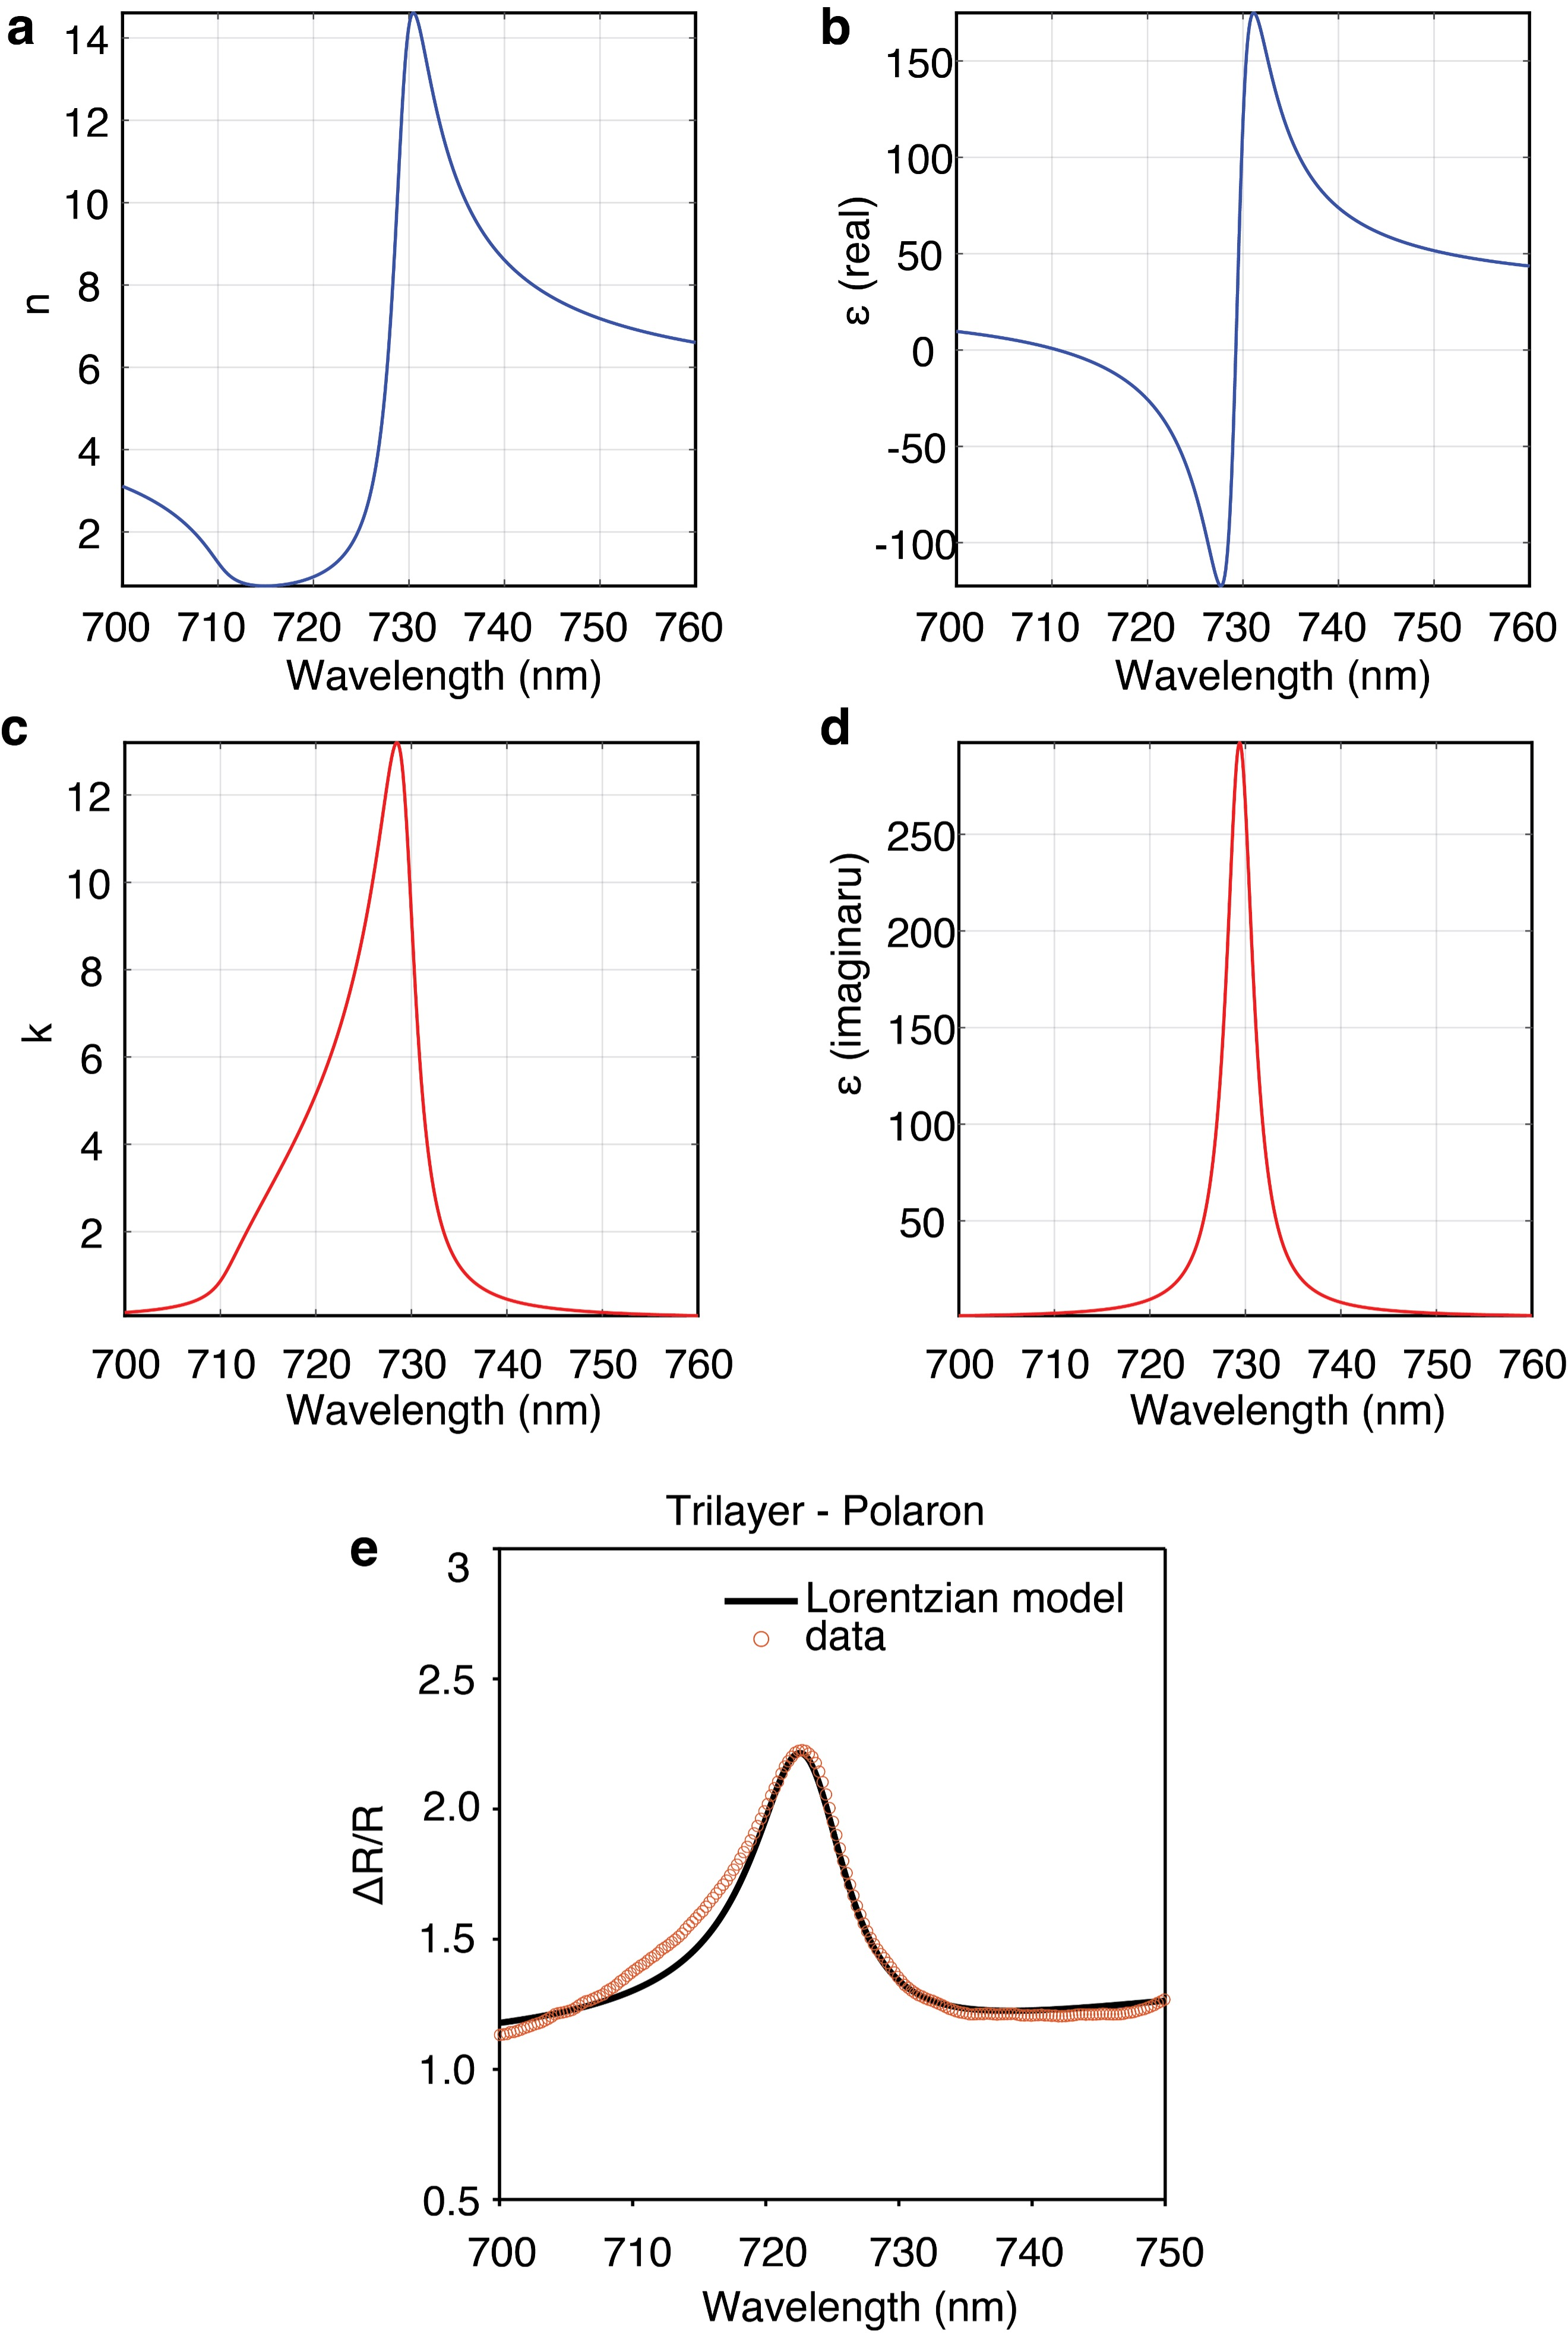
\includegraphics[width=0.65\textwidth]{Figures/C6/Fig6.3.jpg} % 
\end{center}
\caption[Calculated dielectric function and optical index of trilayer WSe$_2$ at $4$ K based on Lorentzian model.] 
{\textbf{Calculated dielectric function and optical index of trilayer WSe$_2$ at $4$ K based on Lorentzian model.}
\textbf{a,b,} Real part of the refractive index and dielectric function. \textbf{c,d,} Imaginary part of the refractive index and dielectric function. \textbf{e,} Comparison of the calculated trilayer WSe$_2$ reflectance and the experimental result.}
\label{fig.6.3}
\end{figure}
\end{quote}
\renewcommand{\baselinestretch}{2}
\small\normalsize
% %/////////////////////// 
When we insert the trilayer WSe$_2$ at the antinodes of the resonant field in the cavity, the exciton resonant with the cavity mode will strongly interact with optical field, leading to a new excitation quasiparticle called polariton. 
The energy of the lower and upper polariton can be derived as Eq.~\ref{eq:LP_UP} as we discussed in \ref{chap4} in the simulation.
Since polaritons are a superposition of the photon and exciton at the same $k_{\parallel}$, 
their fractions of exciton and photon components can be quantified by the squared amplitudes of the Hopfield coefficients $X_{k_{\parallel}}$ and $C_{k_{\parallel}}$. 
In the simulation, the coefficients are calculated based on the Eq.~\ref{eq:Hopcoefficient_Xk} and \ref{eq:Hopcoefficient_Ck}.

Since our objective is to realize nonlinear behavior in the lower polariton, we begin by employing a cavity mode that is resonant with the Fermi polaron(detuning $\Delta$ at zero). 
This configuration maximizes the exciton fraction in the lower polariton branch, thereby providing the most favorable conditions for observing nonlinear effects.

Figure~\ref{fig.6.4} shows the simulated polariton dispersion at $\Delta = 0$, from which we can extract the coupling strength of $\hbar \Omega \sim 42$~meV. While this condition highlights the anti-crossing that defines strong coupling, optimal device performance requires finite detuning. 

%Fig.6.4--------------
% \vspace{1em}
\renewcommand{\baselinestretch}{1}
\small\normalsize
\begin{quote}
\begin{figure}[htbp]
\begin{center}
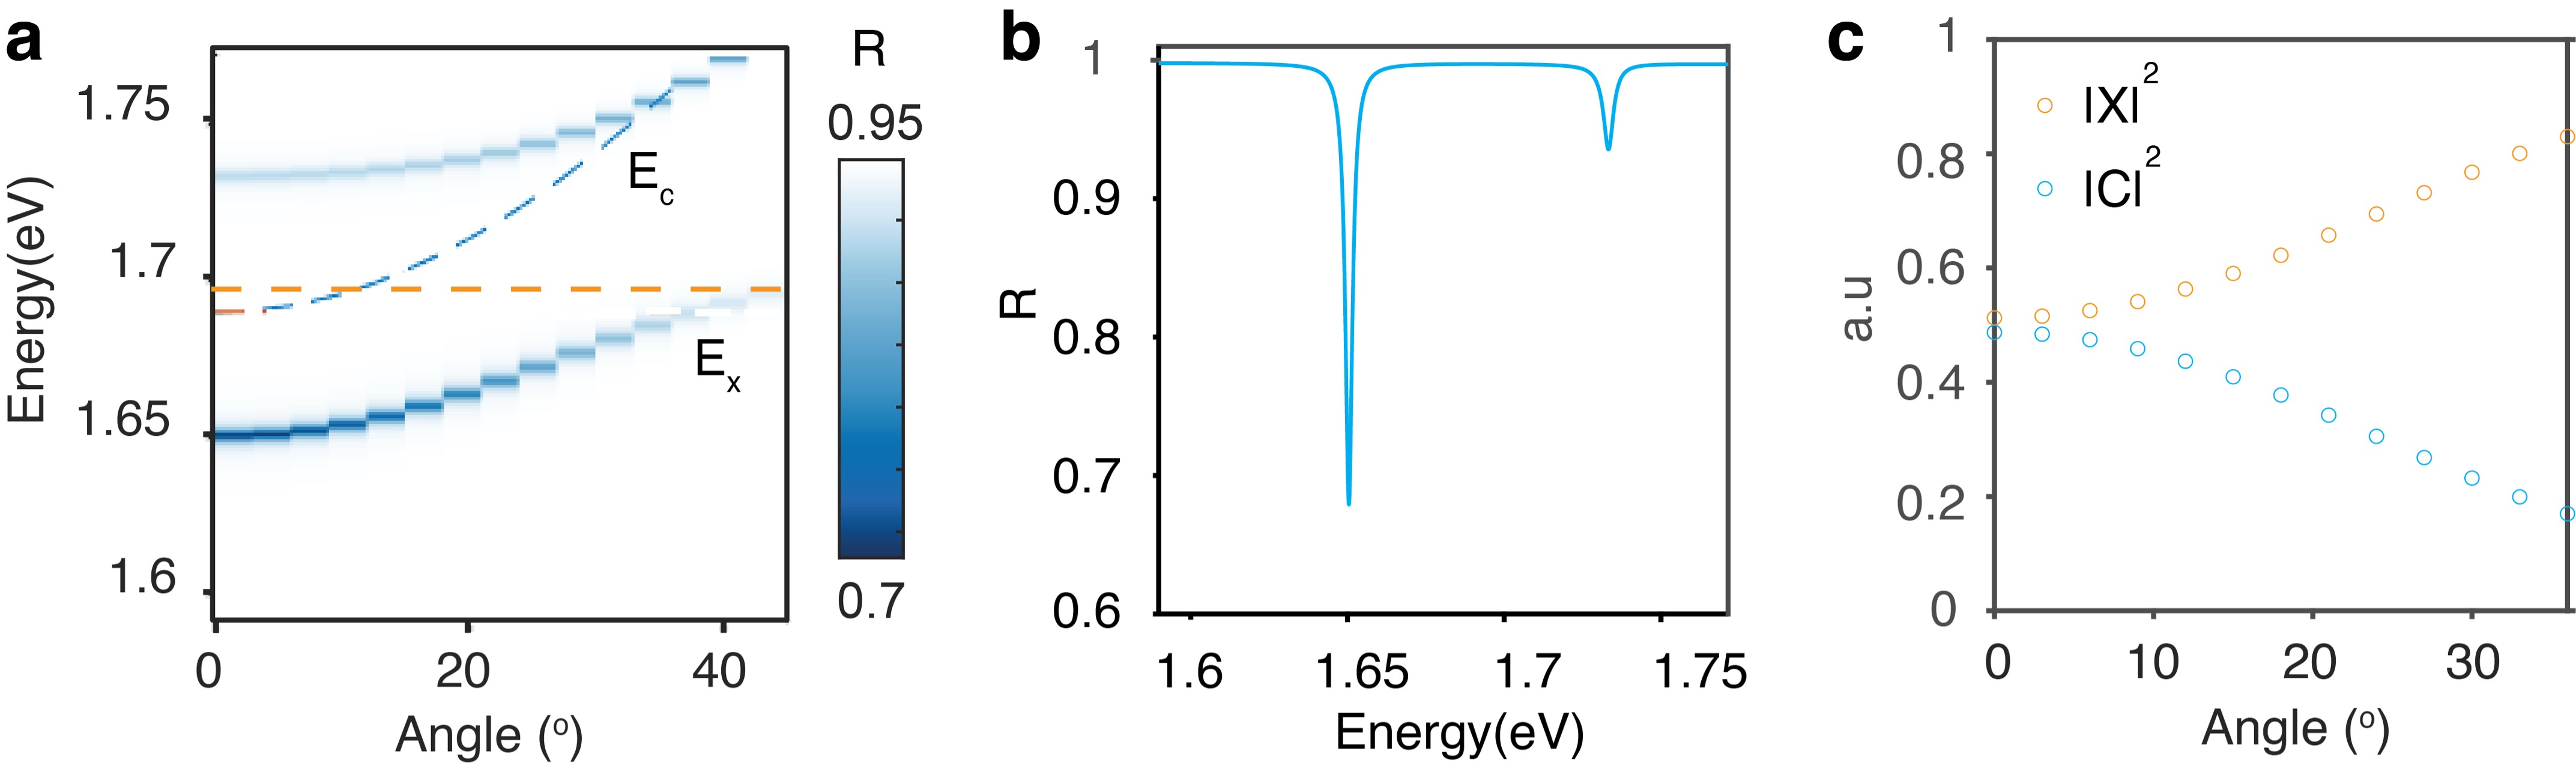
\includegraphics[width=1\textwidth]{Figures/C6/Fig6.4.jpg} % 
\end{center}
\caption[TMM simulation of trilayer WSe$_2$ embedded microcavity reflectance.] 
{\textbf{TMM simulation of trilayer WSe$_2$ embedded microcavity reflectance.}
\textbf{a,}Polariton dispersion at zero detuning ($\Delta = 0$) as a function of incident angle. 
The blue and orange dashed line refers to the cavity and exciton resonance, respectively. 
\textbf{b,} Reflectance spectrum of the polariton at normal incidence. 
\textbf{c,} Calculated Hopfield coefficient of the lower polariton branch.}
\label{fig.6.4}
\end{figure}
\end{quote}
\renewcommand{\baselinestretch}{2}
\small\normalsize
% %/////////////////////// 
Detuning $\Delta$ modifies the relative photon and exciton fractions of the polariton states. 
The polariton’s lifetime primarily inherits from the photon fraction $\lvert C_{k_{\parallel}} \rvert^2$, while nonlinear interactions inherit from the exciton fraction $\lvert X_{k_{\parallel}} \rvert^2$. 
Thus, achieving strong polariton–polariton interactions requires balancing excitonic interaction strength with photonic lifetime. 
This trade-off is quantified by:
$g \sim \lvert X_{k_{\parallel}} \rvert^4 \, U_{\mathrm{ex}}$
where $U_{\mathrm{ex}}$ refers to the exciton–exciton interaction strength. 

We examine a range of detuned conditions by modifying the cavity resonance through both the cavity length (hBN thickness) and the in-plane wavevector $k_{\parallel}$ (as shown in Figure~\ref{fig.6.5}).
According to the simulation results, larger excitonic fractions are obtained only for detuning values $\Delta\geq 0$. The maximum degree of antibunching is expected when the exciton and cavity photon are close to resonance. 
In this case, the required cavity hBN thickness is estimated to be 165–170 nm, corresponding to a cavity resonance near 730 nm. 

%Fig.6.5--------------
% \vspace{1em}
\renewcommand{\baselinestretch}{1}
\small\normalsize
\begin{quote}
\begin{figure}[htbp]
\begin{center}
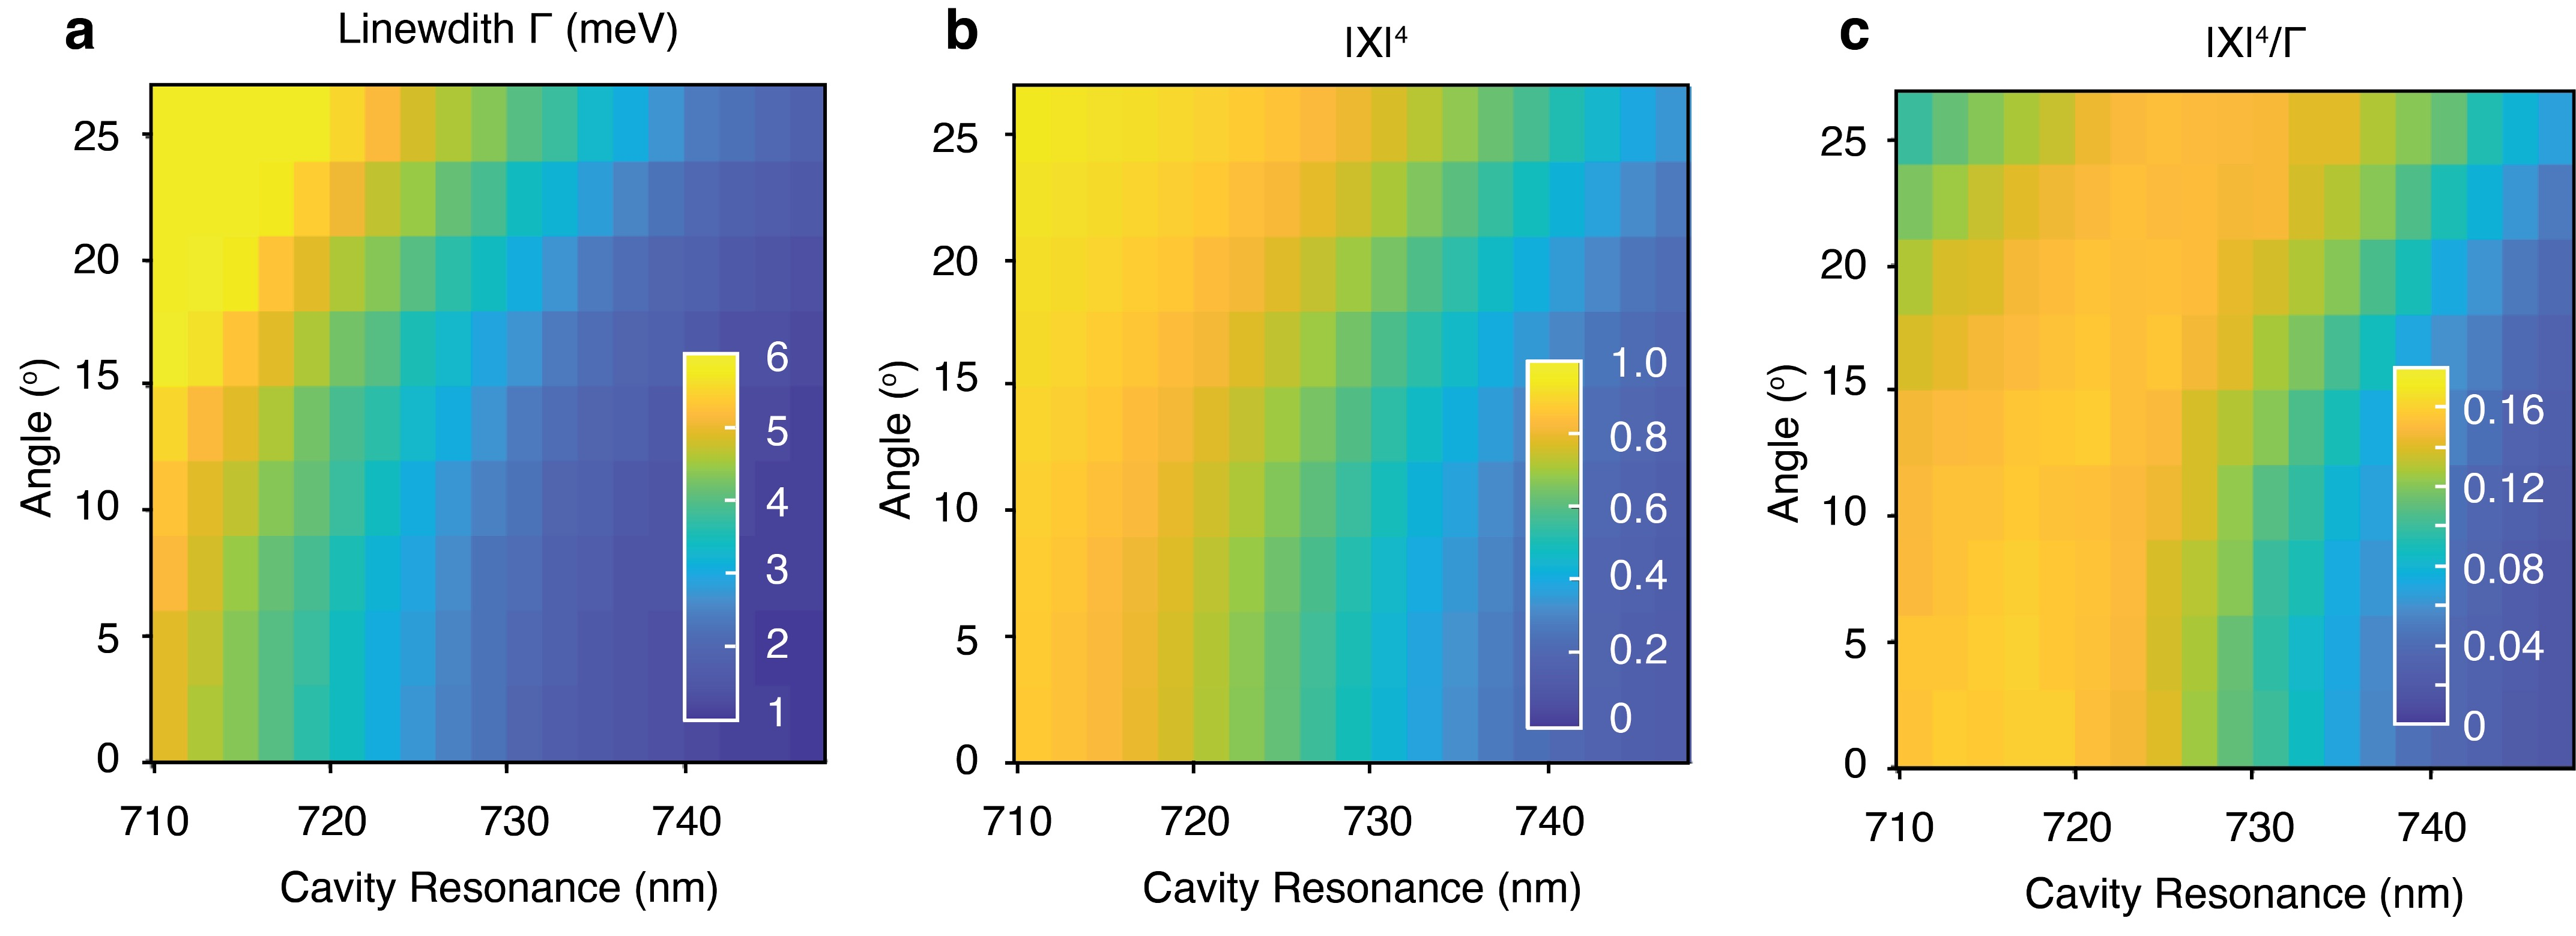
\includegraphics[width=1\textwidth]{Figures/C6/Fig6.5.jpg} % 
\end{center}
\caption[\textit{In situ} tuning lower polariton’s property via detuning $\Delta$.] 
{\textbf{\textit{In situ} tuning lower polariton’s property via detuning $\Delta$.}
\textbf{a}, Linewidth of the lower polariton as a function of cavity resonance and angle. 
\textbf{b}, Excitonic contribution $\lvert X_{k_{\parallel}} \rvert^4$ extracted from the Hopfield coefficient. 
\textbf{c}, Effective interaction strength parameter $\lvert X_{k_{\parallel}} \rvert^4 / \Gamma$ indicating the maximum degree of antibunching.
}
\label{fig.6.5}
\end{figure}
\end{quote}
\renewcommand{\baselinestretch}{2}
\small\normalsize
% %/////////////////////// 

\section{Sample Fabrication}
We used a bottom DBR stack comprising 12.5 pairs of TiO$_2$/SiO$_2$ films with alternating thicknesses of 340~nm/120~nm sputtered on 285~nm SiO$_2$/Si. 
This combination produces a stopband between 710--780~nm. 
Graphite and hBN flakes were then mechanically exfoliated from bulk crystals onto the silicon chip with a SiO$_2$ layer. 
The thickness of each layer was identified using Atomic Force Microscopy (AFM). 
Based on our Transfer Matrix Method (TMM) simulation, we selected 80~nm hBN (Device~1) / 90~nm hBN (Device~2) as the top and bottom encapsulation, which yields a cavity resonance close to the Fermi polaron. 
Monolayer graphene / bilayer graphite was chosen for the top and bottom gates due to the strong absorption of thick graphite in the visible range. 

The van der Waals heterostructures were assembled using a dry-transfer method with PDMS (polydimethylsiloxane) and PC (polycarbonate) as the stamp, sequentially stacking all the flakes onto the bottom DBR substrate. 
Electrical contacts were then defined by electron-beam lithography, followed by a liftoff process after thermal evaporation of 5~nm Cr and 100~nm Au. 
Finally, the silver top mirror (35--40~nm thick) was patterned using the same lithography and liftoff procedure. 
During the electron-beam lithography step for the silver mirror, a low beam current of 300~pA was employed to minimize potential degradation of the optical properties of the trilayer WSe$_2$ in the active region.
Figures~\ref{fig.6.6} shows the optical image of the fabricated devices.
Figures~\ref{fig.6.7} shows the device schematic and the simulated reflectace spectrum for D1 and D2.

%Fig.6.6--------------
% \vspace{1em}
\renewcommand{\baselinestretch}{1}
\small\normalsize
\begin{quote}
\begin{figure}[htbp]
\begin{center}
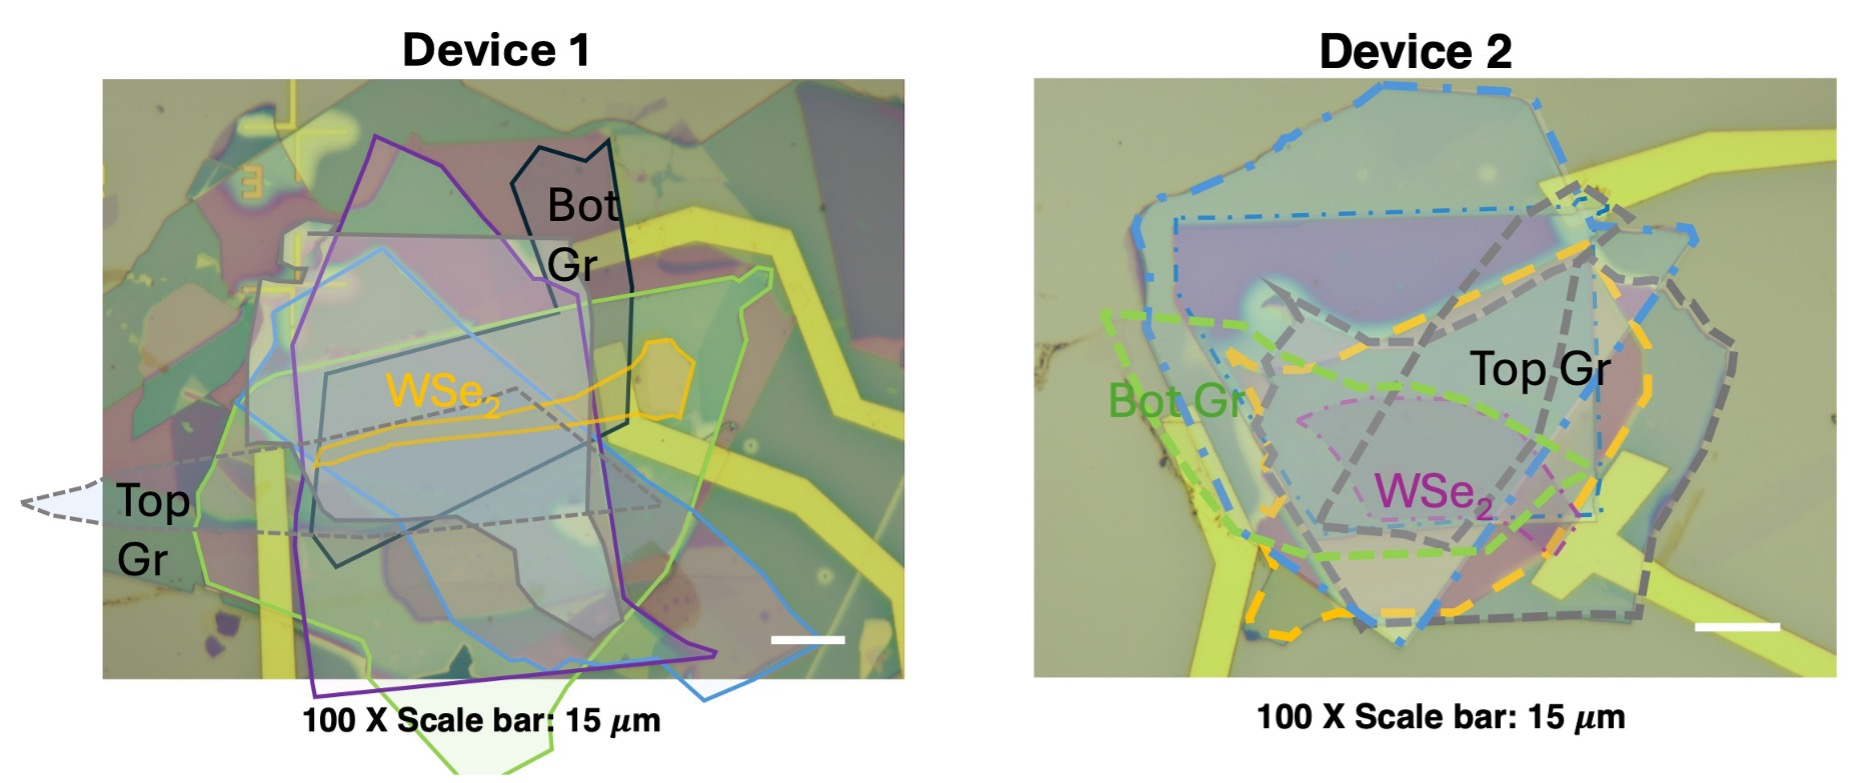
\includegraphics[width=1\textwidth]{Figures/C6/Fig6.6.jpg} % 
\end{center}
\caption[Optical image of the van der Waals microcavity Device 1 and 2 (without Ag)] 
{\textbf{Optical image of the van der Waals microcavity Device 1 and 2 (without Ag)}
}
\label{fig.6.6}
\end{figure}
\end{quote}
\renewcommand{\baselinestretch}{2}
\small\normalsize
% %/////////////////////// 
%Fig.6.7--------------
% \vspace{1em}
\renewcommand{\baselinestretch}{1}
\small\normalsize
\begin{quote}
\begin{figure}[htbp]
\begin{center}
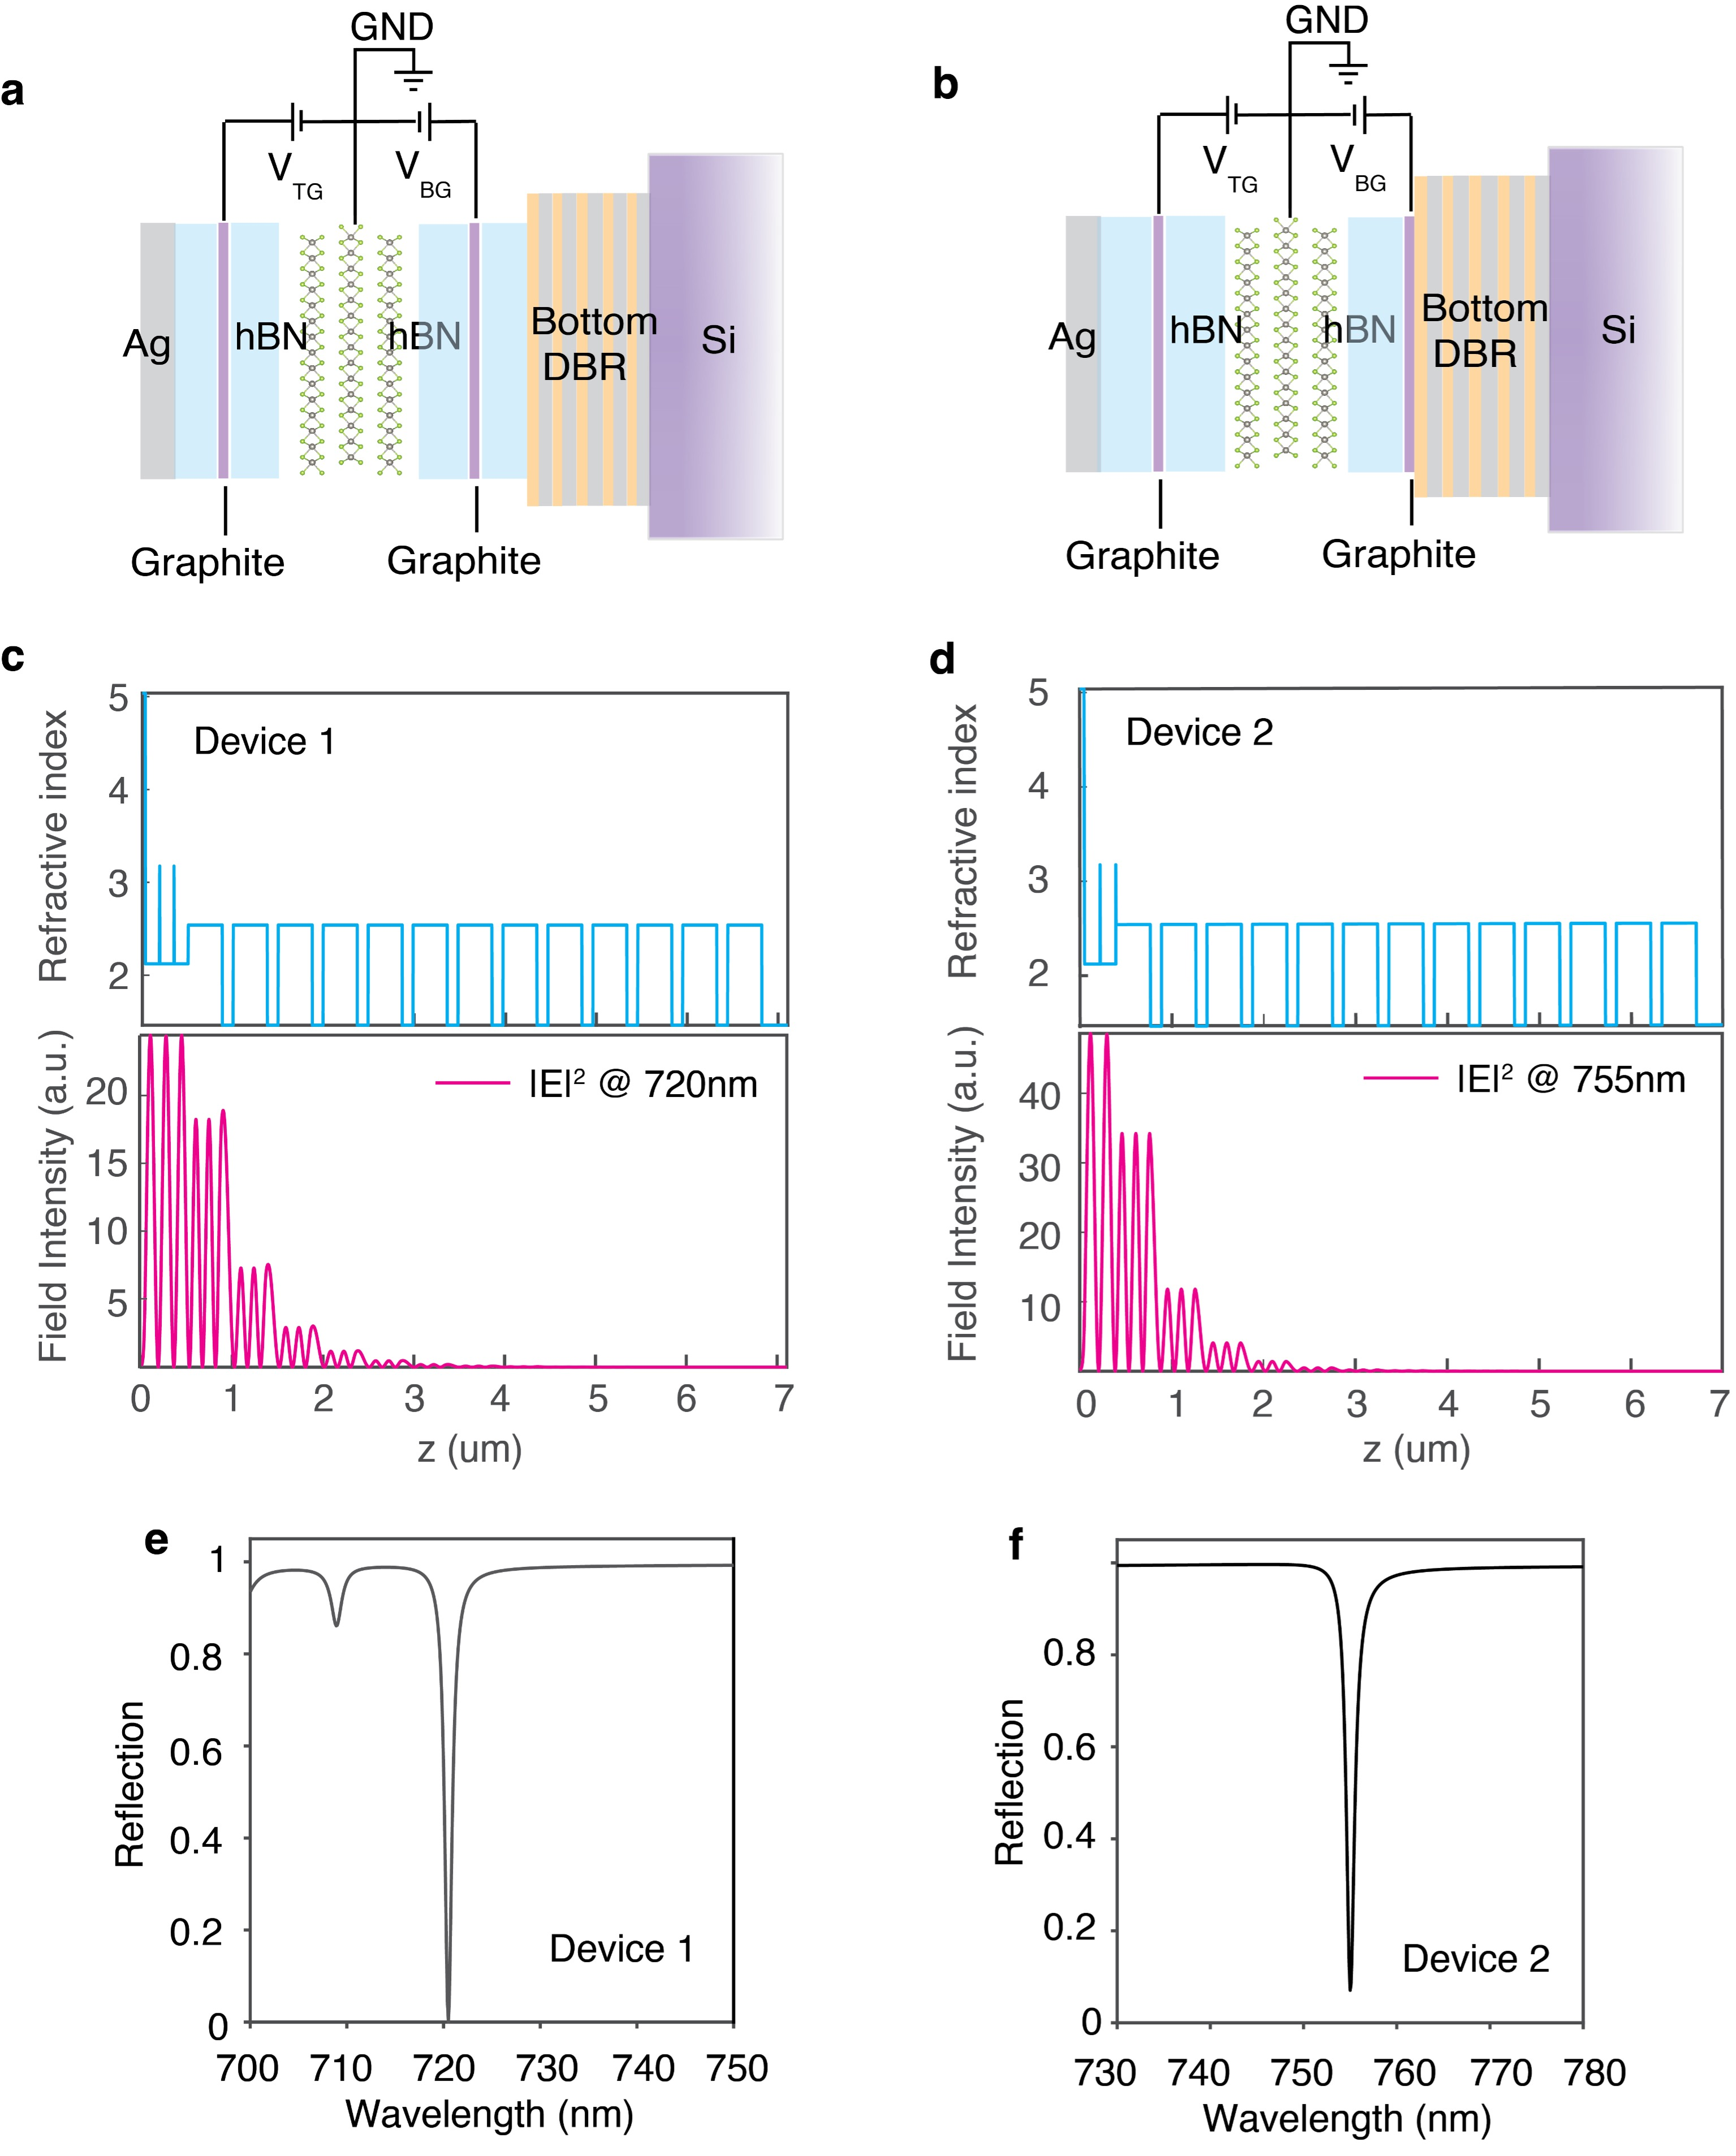
\includegraphics[width=0.8\textwidth]{Figures/C6/Fig6.7.jpg} % 
\end{center}
\caption[TMM Simulation of the Ag/DBR microcavity resonance for D1 and D2.] 
{\textbf{TMM Simulation of the Ag/DBR microcavity resonance for D1 and D2.}
\textbf{a, b,} Schematic of D1 and D2. \textbf{c, d,} Corresponded cavity structure and field intensity distribution $|E|^2$. In D1 there are in total three modes within the cavity, while in D2 there are two. 
However, the thinner cavity length structure should simplifier fabrication process, thus may lead to higher quality. \textbf{e, f,} Simulated cavity resonance. The linewidth is $\sim$ 0.7 nm for both resonances. 
}
\label{fig.6.7}
\end{figure}
\end{quote}
\renewcommand{\baselinestretch}{2}
\small\normalsize
% %/////////////////////// 

\section{Results and Discussions}
The cavity resonance of the first device D1 is designed for on resonantly couple to the exciton X$_A$ of the monolayer WSe$_2$ and slightly blue-detuned to the polaron in trilayer WSe$_2$. 
The cavity resonance of the second device D2 is designed red detuned to the trilayer WSe$_2$ polaron ($\Delta = -2 \hbar \Omega$). 
We first characterize the resonant energy and quality factor of the bare cavity, prior to the introduction of the monolayer or trilayer WSe$_2$. 
Due to the inherent inhomogeneity in the 2D stack, the linewidth of the cavity mode can be as narrow as 4 nm, corresponding to a quality factor of approximately 182.5.

\subsection{k-space imaging of the polariton dispersion in monolayer/ trilayer WSe$_2$}
To investigate exciton--polariton formation, we performed angle-resolved reflection imaging on both monolayer and trilayer WSe$_2$ embedded in the optical cavity in D1. 
Clear signatures of strong coupling between excitons and cavity photons were observed in both regions (see Figure~\ref{fig.6.8}). 
By fitting the upper and lower polariton with a coupled oscillator model, we extract the coupling strength $\hbar \Omega$ (half of the Rabi splitting) based on the Eq.~\ref{eq:LP_UP}.

% %/////////////////////// 
%Fig.6.7--------------
% \vspace{1em}
\renewcommand{\baselinestretch}{1}
\small\normalsize
\begin{quote}
\begin{figure}[htbp]
\begin{center}
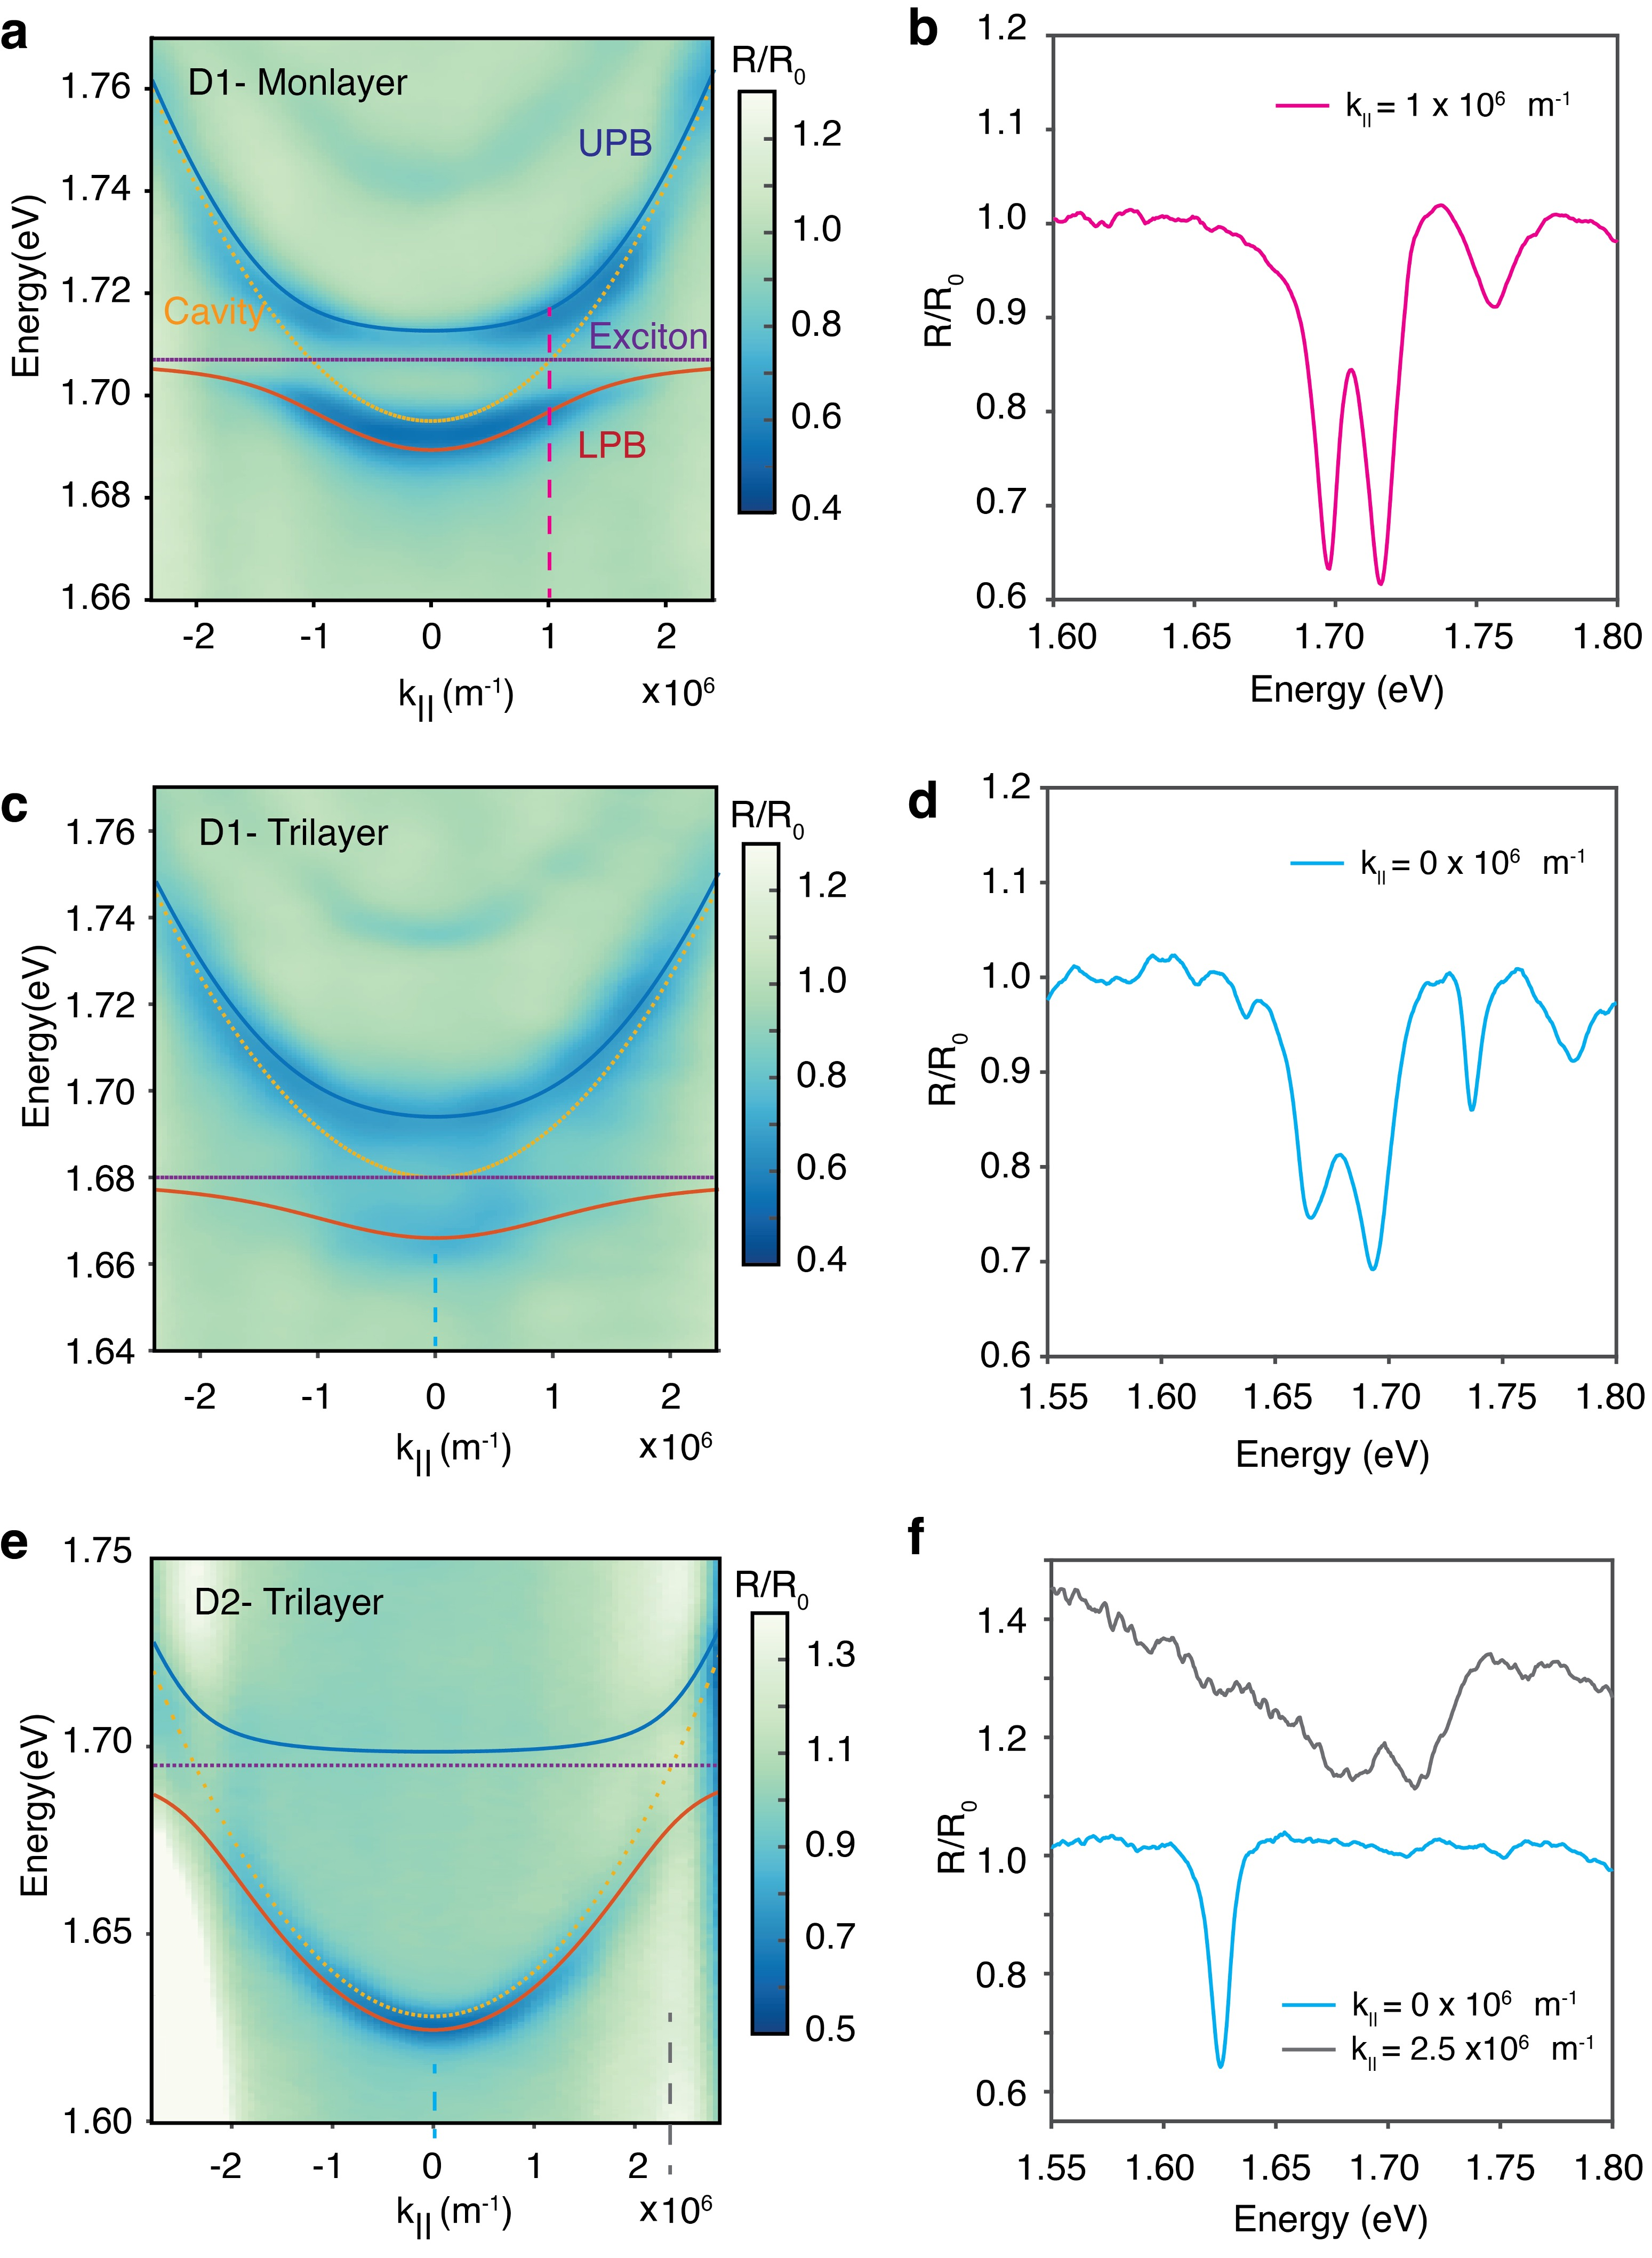
\includegraphics[width=0.8\textwidth]{Figures/C6/Fig6.8.jpg} % 
\end{center}
\caption[Strong coupling of exciton/polaron-polaritons in monolayer and trilayer WSe$_2$.] 
{\textbf{Strong coupling of exciton/polaron-polaritons in monolayer and trilayer WSe$_2$.}
\textbf{a}, Angle-resolved reflectance spectrum of exciton polaritons in D1 monolayer WSe$_2$ ($\Delta>0$).  
\textbf{c}, D1 trilayer WSe$_2$ ($\Delta=0$).  
\textbf{e}, D2 trilayer WSe$_2$ ($\Delta<0$).  
The blue and red solid lines show the fitted upper and lower polariton modes. 
The yellow dotted line corresponds to the cavity mode dispersion, and the purple dotted line marks the exciton energy.  
\textbf{b}, Reflectance spectrum of D1 monolayer at the anti-crossing position indicated by the magenta dashed line in (a).  
The energy splitting between LPB and UPB is $2\hbar\Omega \approx 20 \pm 1$~meV.  
\textbf{d}, Reflectance spectrum of D1 trilayer at $k_{\parallel}=0$ (where $E_{\mathrm{exc}} = E_{\mathrm{ph}}$), indicated by the blue dashed line in (c).  
The energy splitting between LPB and UPB is $2\hbar\Omega \approx 30 \pm 2$~meV.  
\textbf{f}, Reflectance spectrum of D2 trilayer at $k_{\parallel}=0$ (blue solid line) and at the anti-crossing region where $E_{\mathrm{exc}} = E_{\mathrm{ph}}$ (gray solid line).  
The energy splitting between LPB and UPB is $2\hbar\Omega \approx 33 \pm 3$~meV.
}
\label{fig.6.8}
\end{figure}
\end{quote}
\renewcommand{\baselinestretch}{2}
\small\normalsize
% %/////////////////////// 

For the monolayer, we obtained a coupling strength of about 10~meV for $\hbar\Omega$, while in the trilayer the value increases to $\sim$15~meV.
Given the cavity linewidth $\gamma_{\mathrm{cav}}$ (6--10~meV) and the polaron linewidth $\gamma_{\mathrm{polaron}}$ ($\sim$10~meV), these values satisfy the strong-coupling condition, $2\hbar\Omega > \gamma_{\mathrm{cav}} + \gamma_{\mathrm{polaron}}$.
Meeting this criterion confirms that the system supports polaritons as the new eigenmodes, as evidenced experimentally by the anti-crossing in the dispersion.
By contrast, in the weak-coupling regime the anti-crossing would be absent, and the exciton and photon resonances would remain uncoupled.

The stronger coupling observed in the trilayer can be attributed to the collective nature of light–matter interaction.
In multilayer structures, the vacuum Rabi splitting scales with the total oscillator strength coupled to the mode, which increases with the number of active layers $N$ if assuming uniform field overlap.
A standard approximation in multiple–quantum-well microcavities gives:
\begin{equation}
\hbar\Omega \sim \sqrt{\frac{N f}{L_{\mathrm{eff}}}}
\label{eq:Rabi_layers}
\end{equation}
where $f$ is the per-layer oscillator strength of the active transition and $L_{\mathrm{eff}}$ is the optical length of the cavity~\cite{ref41}.
This takes the same form as Eq.~\eqref{eq:rabi}.
This therefore predicts a square-root dependence of $\hbar\Omega$ on the number of embedded layers, so a trilayer ($N=3$) naturally exhibits a larger splitting than a monolayer ($N=1$).

This square-root scaling is well established in strongly coupled systems such as GaAs and CdTe multiple–quantum-well microcavities, where collective enhancement from multiple wells boosts the light–matter interaction.
The same principle applies to TMDs: the trilayer exhibits enhanced coupling because the effective oscillator strength is multiplied by the number of coupled layers.

Furthermore, in the trilayer region the exciton resonance (1.69~eV) lies close to the cavity photon energy, which causes the upper polariton branch to remain near the bare cavity dispersion while the lower polariton branch follows the excitonic dispersion, consistent with the measured anti-crossing.

\subsection{Electrically tunable exciton/polaron-polaritons in monolayer and trilayer WSe$_2$}
Electrical control of van der Waals heterostructures enables dynamic tuning of many-body interactions in TMD layers, giving rise to the formation of exciton–polarons.
Because polaritons inherit the intrinsic properties of their excitonic component, electrical gating serves as an effective knob to modulate their dispersion, composition, and nonlinear response.
Such tunability offers a pathway toward reconfigurable polaritonic devices, where propagation, confinement, and interaction strength can be actively controlled without altering the cavity structure.

To investigate these effects, we measured gate-dependent reflectance to access the polaron – polariton states.
For more efficient and uniform doping, a halogen lamp was used to illuminate a large area of the sample, thereby enhancing charge transfer at the locally probed spot during gating.
In the monolayer region, as shown in Figure~\ref{fig.6.9}a, the two polariton branches exhibit smooth energy blueshifts under intrinsic and low-doping conditions.
This behavior arises from phase-space filling of the repulsive polaron in monolayer WSe$_2$ under doping.
At higher hole-doping levels, attractive polaron–polaritons emerge, but with a reduced energy splitting ($\sim$13~meV) compared to the intrinsic case ($\sim$22~meV).

% %/////////////////////// 
%Fig.6.9--------------
% \vspace{1em}
\renewcommand{\baselinestretch}{1}
\small\normalsize
\begin{quote}
\begin{figure}[htbp]
\begin{center}
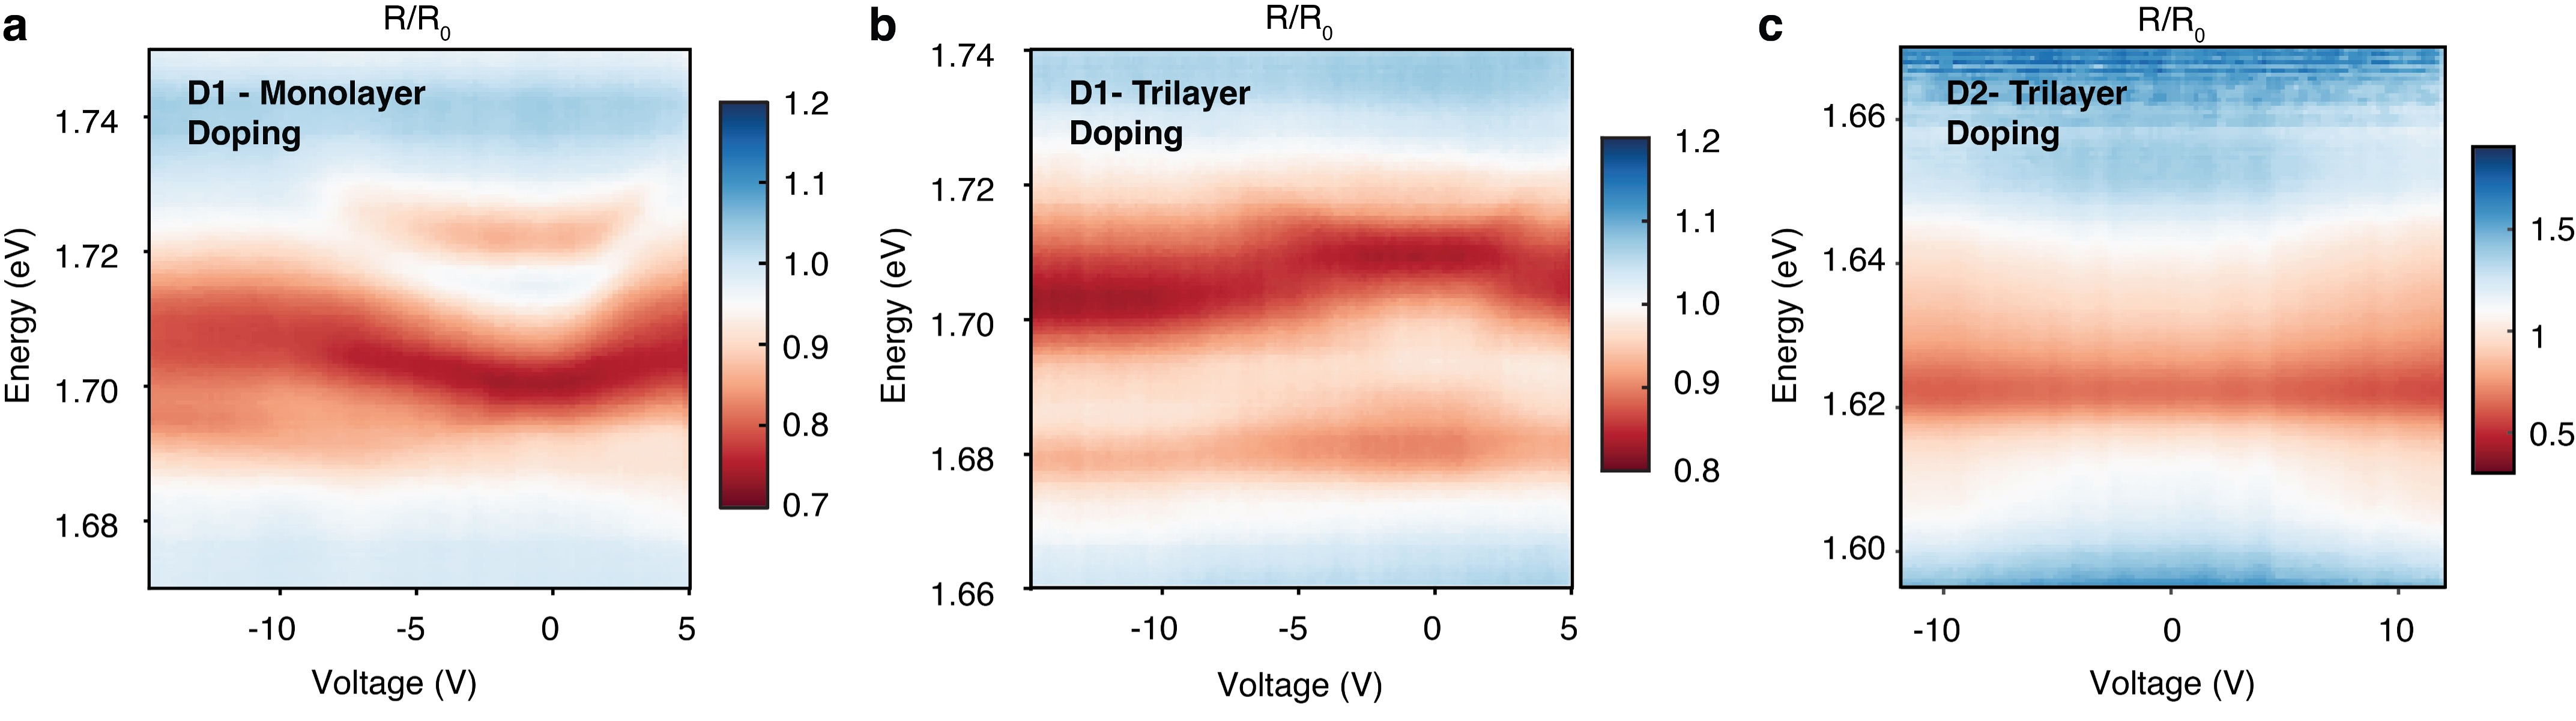
\includegraphics[width=1\textwidth]{Figures/C6/Fig6.9.jpg} % 
\end{center}
\caption[Doping dependent map of reflectance at 5 K.] 
{\textbf{Doping dependent map of reflectance at 5 K.}
Normalized reflectance as a function of gate voltage in \textbf{a,} monolayer and \textbf{b,} trilayer WSe$_2$ in D1, \textbf{c,} trilayer WSe$_2$ in D2.
} 
\label{fig.6.9}
\end{figure}
\end{quote}
\renewcommand{\baselinestretch}{2}
\small\normalsize
% %/////////////////////// 
In contrast, in the trilayer WSe$_2$ region of D1, we observe consistently large Rabi splittings across all gating regimes, with an exciton–polariton splitting of $\sim$ 30.5~meV and a polaron–polariton splitting of $\sim$ 28.3~meV.  
The persistence of large energy splittings under all electrical gating conditions in the trilayer region is expected, since polarons in trilayers possess larger oscillator strength and therefore couple more strongly to the cavity photon.  

By comparison, in the D2 trilayer WSe$_2$ region with detuning $\Delta \sim -2\hbar\Omega$, the lower polariton branch has a high photon fraction and is therefore expected to show minimal gate dependence.  
Experimentally, we indeed observe only a broadening of the dip feature with increasing gate voltage, which can be attributed to linewidth broadening of the polaron species arising from exciton–carrier scattering.

\subsection{Distinct polariton nonlinear behavior with power}
Next, we studied the polariton nonlinear behavior in the monolayer and trilayer regions in D1. 
A supercontinuum white laser was used for broadband power dependent reflection measurements, with the wavelength range selected by an acousto-optic tunable filter (AOTF): 715–755 nm for the trilayer region and 715–750 nm for the monolayer region (see in Figure~\ref{fig.6.10}).

% %/////////////////////// 
%Fig.6.10--------------
% \vspace{1em}
\renewcommand{\baselinestretch}{1}
\small\normalsize
\begin{quote}
\begin{figure}[htbp]
\begin{center}
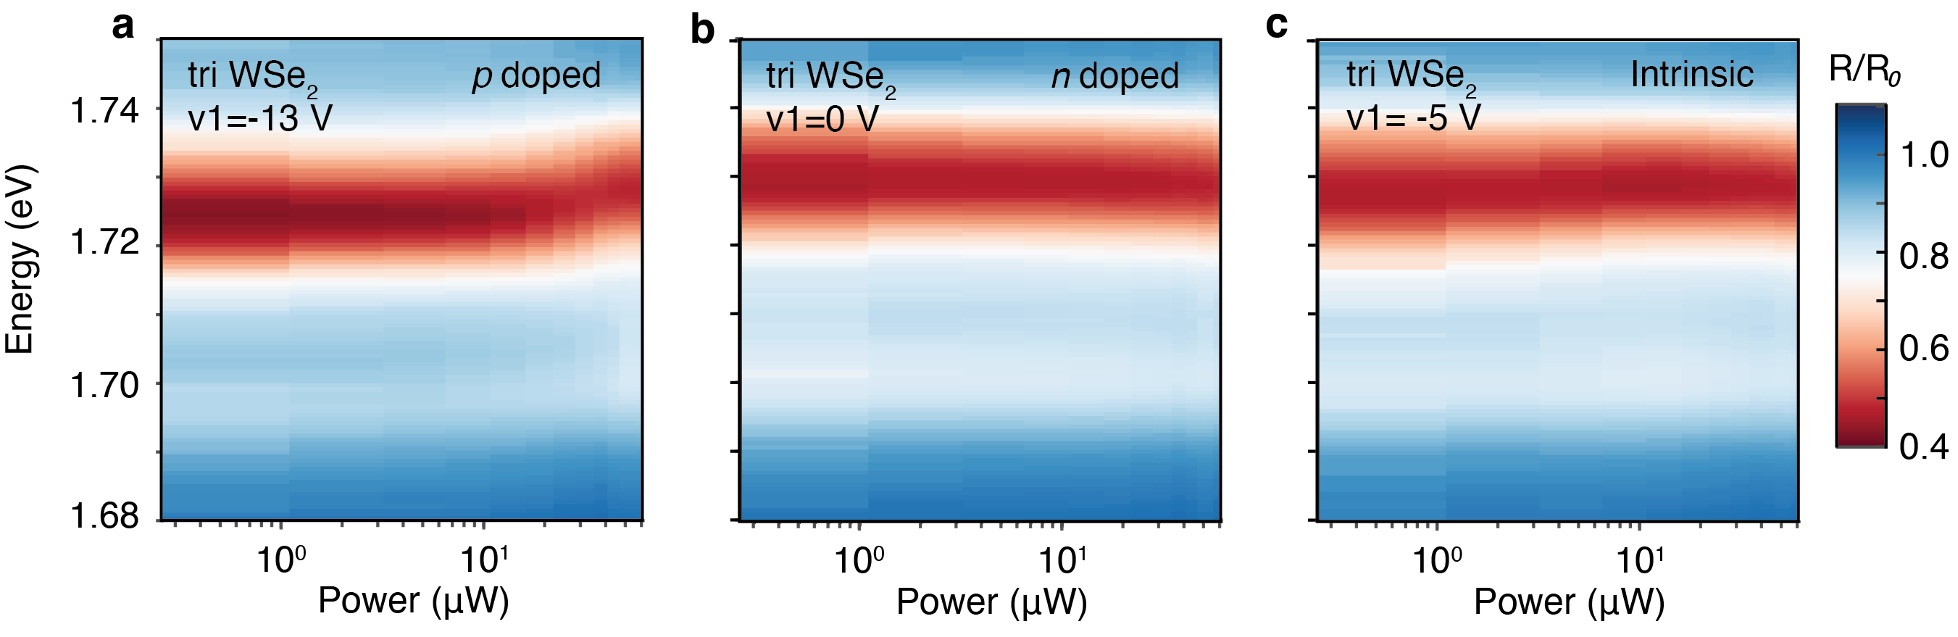
\includegraphics[width=1\textwidth]{Figures/C6/Fig6.10.jpg} % 
\end{center}
\caption[Power dependent reflectance of polaritons in trilayer WSe$_2$.] 
{\textbf{Power dependent reflectance of polaritons in trilayer WSe$_2$.}
\textbf{a,} LP and UP polaron polariton energy blueshift as a function of the pulsed laser excitation average power (715-755 nm). Both the polariton species shows an energy blueshift with power, while for the \textbf{b,} electron dope and \textbf{c,} intrinsic case this nonlinear behavior is absent.
} 
\label{fig.6.10}
\end{figure}
\end{quote}
\renewcommand{\baselinestretch}{2}
\small\normalsize
% %/////////////////////// 
In the trilayer region, we compared two doping conditions at: intrinsic (V1 = -5 V) and hole doped side (V1 = -13V). 
This nonzero voltage corresponded intrinsic case is due to the inefficient doping across the sample by using the supercontinuum laser as a small excitation spot. 
Under hole doping, both polariton branches exhibited energy blueshifts with increasing excitation power: the lower polariton shifted by ~4.3 meV, while the upper branch shifted by ~3.8 meV.
The difference in blueshift can be attributed to the unequal exciton fractions in the LPB and UPB, since the nonlinear interaction between the polaritons contributed from the excitonic part scales as $\lvert X_{(k_{\parallel})} \rvert^{4} \cdot g_{\mathrm{exc}}$. 
In contrast, under intrinsic doping, only the upper branch showed an energy redshift of about 1.2 meV, while the lower branch exhibited no significant change.

In the monolayer region, within the same power range, no energy shift was observed. 
However, when we further increased both the excitation power and the laser bandwidth, the lower and upper polariton energies shifted toward each other. 
This behavior is consistent with phase space filling induced polariton nonlinearity: at high non-resonant excitation power, 
the exciton density increases, and phase-space filling reduces the available oscillator strength, weakening the light–matter coupling and thereby decreasing the Rabi splitting.

We then quantitatively analyzed the photon flux required to induce the observed polariton shift and compared it with the polaron nonlinearity. 
For an excitation bandwidth of 715--755~nm, a lower polariton blueshift of 4.3~meV corresponded to approximately $2.5 \times 10^{5}$ photons per~$\mu$m$^{2}$. 
In homotrilayer WSe$_2$, a comparable nonlinear shift ($\sim$4~meV) was observed at a similar photon flux. 
However, due to the large cavity leakage (cavity mode FWHM $\sim$10~nm), the polariton linewidth ($\sim$16~meV) is significantly broader than the polaron linewidth ($\sim$10~meV). 
In this case, the polariton linewidth is primarily limited by the cavity quality.

\section{Summary and Outlook}
In summary, we fabricated electrically tunable one-dimensional microcavity with trilayer WSe$_2$ van der Waals heterostructures embedded. 
By varying the thickness of the encapsulating hBN layers, we achieved different detuning $\Delta$ conditions at zero in-plane wavevector. 
At $T = 5$~K, we observed strong coupling between excitons/polarons and cavity photons, as evidenced by the formation of lower and upper polaritons. 
Angle-resolved reflectivity measurements revealed clear anti-crossing behavior between the polariton branches. 
The extracted Rabi splitting of the exciton–polariton in the trilayer was approximately 30~meV, significantly larger than the 20~meV splitting observed in the monolayer, which is due to the enhanced oscillator strength of excitons/polarons in the trilayer. 
Notably, strong coupling persists across a wide range of gate voltages in trilayers, in contrast to the monolayer case, where it disappears under similar conditions.  

Under resonant excitation of the polariton modes in trilayer WSe$_2$, we observed clear nonlinear responses in the weak-pump regime. 
In the hole-doped case, both the lower and upper polariton branches exhibited energy blueshifts with increasing pump power, whereas no such shifts were detected under intrinsic or electron-doped conditions. 
This behavior is consistent with polaron-mediated interactions in homotrilayer WSe$_2$, indicating that excitonic interactions dominate the polariton nonlinearity at low excitation densities. 
At higher pump powers, the Rabi splitting progressively decreased, which we attribute to phase-space filling effects that reduce the available excitonic oscillator strength and weaken the light–matter coupling.  

Overall, our results demonstrate that polaron–polaritons in trilayer WSe$_2$ combine strong oscillator strength with pronounced optical nonlinearities under hole doping. 
These properties establish trilayer WSe$_2$ microcavities as a promising platform for exploring bright, strongly interacting polariton systems, and for advancing towards the quantum nonlinear regime, where phenomena such as polariton blockade and strongly correlated photonic states are anticipated.
